\documentclass[a4paper, twoside]{report}

%% Language and font encodings
\usepackage[english]{babel}
\usepackage[utf8x]{inputenc}
\usepackage[T1]{fontenc}

%% Sets page size and margins
\usepackage[a4paper,top=3cm,bottom=2cm,left=3cm,right=3cm,marginparwidth=1.75cm]{geometry}

%% Useful packages
\usepackage{amsmath}
\usepackage{mathtools}
\usepackage{amssymb}
\usepackage{graphicx}
\usepackage{listings}
\usepackage{float}
\usepackage{xcolor}
\usepackage[colorinlistoftodos]{todonotes}
\usepackage[colorlinks=true, allcolors=blue]{hyperref}

% Code blocks
\definecolor{dkgreen}{RGB}{0,128,0} % Define the dkgreen color using RGB values
\lstset{
  frame=none,
  language=Promela,
  aboveskip=5mm,
  belowskip=5mm,
  showstringspaces=false,
  columns=flexible,
  xleftmargin=.3\textwidth,
  basicstyle={\small\ttfamily},
  numbers=none,
  numberstyle=\tiny\color{gray},
  keywordstyle=\color{blue},
  commentstyle=\color{dkgreen},
  stringstyle=\color{orange},
  breaklines=true,
  breakatwhitespace=true,
  tabsize=3,
  numbers=left, 
  captionpos=b, 
}

% Elixir code colouring
\definecolor{commentgreen}{RGB}{2,112,10}
\definecolor{eminence}{RGB}{108,48,130}
\definecolor{weborange}{RGB}{255,165,0}
\definecolor{frenchplum}{RGB}{129,20,83}

\lstdefinelanguage{elixir}{
    morekeywords={case,catch,def,do,else,false,%
        use,alias,receive,timeout,defmacro,defp,%
        for,if,import,defmodule,defprotocol,%
        nil,defmacrop,defoverridable,defimpl,%
        super,fn,raise,true,try,end,with,%
        unless, quote, unquote},
    otherkeywords={<-,->, |>, \%\{, \}, \{, \, (, )},
    sensitive=true,
    morecomment=[l]{\#},
    morecomment=[n]{/*}{*/},
    morecomment=[s][\color{purple}]{:}{\ },
    morestring=[s][\color{orange}]"",
    commentstyle=\color{commentgreen},
    keywordstyle=\color{eminence},
    stringstyle=\color{red},
	basicstyle=\ttfamily,
	breaklines,
	showstringspaces=false,
	frame=none
}
\lstdefinelanguage{dafny}{
    morekeywords={method, function, class, var, assert, ensures, requires, modifies, decreases, new, if, else, while, break, return, ghost, forall, exists, invariant, axiom, datatype},
    sensitive=true,
    morecomment=[l]{//},
    morecomment=[s]{/*}{*/},
    morestring=[b]",
    commentstyle=\color{green},
    keywordstyle=\color{blue},
    stringstyle=\color{red},
    basicstyle=\ttfamily,
    breaklines,
    showstringspaces=false,
    frame=none
}
\lstdefinelanguage{boogie}{
    morekeywords={implementation, procedure, assert, assume, havoc, call, return, var, function, modifies, ensures, requires, if, else, while, break, continue},
    sensitive=true,
    morecomment=[l]{//},
    morecomment=[s]{/*}{*/},
    morestring=[b]",
    commentstyle=\color{green},
    keywordstyle=\color{blue},
    stringstyle=\color{red},
    basicstyle=\ttfamily,
    breaklines,
    showstringspaces=false,
    frame=none
}
\lstdefinelanguage{none}{}

\title{Verification Aware Elixir (Interim Report)}
\author{Matthew Neave}
% Update supervisor and other title stuff in title/title.tex

\begin{document}
\begin{titlepage}

\newcommand{\HRule}{\rule{\linewidth}{0.5mm}} % Defines a new command for the horizontal lines, change thickness here

%----------------------------------------------------------------------------------------
%	LOGO SECTION
%----------------------------------------------------------------------------------------


\includegraphics[width=8cm]{title/logo.eps}\\[1cm] % Include a department/university logo - this will require the graphicx package
 
%----------------------------------------------------------------------------------------

\center % Center everything on the page

%----------------------------------------------------------------------------------------
%	HEADING SECTIONS
%----------------------------------------------------------------------------------------

\textsc{\LARGE MEng Individual Project}\\[1.5cm] % Name of your university/college
\textsc{\Large Imperial College London}\\[0.5cm] % Major heading such as course name
\textsc{\large Department of Computing}\\[0.5cm] % Minor heading such as course title

%----------------------------------------------------------------------------------------
%	TITLE SECTION
%----------------------------------------------------------------------------------------
\makeatletter
\HRule \\[0.4cm]
{ \huge \bfseries \@title}\\[0.4cm] % Title of your document
\HRule \\[1.5cm]
 
%----------------------------------------------------------------------------------------
%	AUTHOR SECTION
%----------------------------------------------------------------------------------------

\begin{minipage}{0.4\textwidth}
\begin{flushleft} \large
\emph{Author:}\\
\@author % Your name
\end{flushleft}
\end{minipage}
~
\begin{minipage}{0.4\textwidth}
\begin{flushright} \large
\emph{Supervisor:} \\
Dr. Naranker Dulay \\[1.2em] % Supervisor's Name
\emph{Second Marker:} \\
TBD % second marker's name
\end{flushright}
\end{minipage}\\[2cm]
\makeatother

% If you don't want a supervisor, uncomment the two lines below and remove the section above
%\Large \emph{Author:}\\
%Matthew \textsc{Neave}\\[3cm] % Your name

%----------------------------------------------------------------------------------------
%	DATE SECTION
%----------------------------------------------------------------------------------------

{\large \today}\\[2cm] % Date, change the \today to a set date if you want to be precise

\vfill % Fill the rest of the page with whitespace

\end{titlepage}

\begin{abstract}
Your abstract goes here
\end{abstract}

\renewcommand{\abstractname}{Acknowledgements}
\begin{abstract}
Thanks mum!
\end{abstract}

\tableofcontents
\listoffigures
\listoftables

\chapter{Introduction}
With the rise of cloud-based clusters, developing robust distributed algorithms is becoming an increasingly difficult problem and the need for vigorous methodologies to verify the correctness of these algorithms has intensified. Modern programming languages have been developed to support distributed algorithms that rely on message-passing as a means of communication between sequential nodes executing in parallel. Common message-passing abstractions involve the use of channels (e.g. Go \cite{go}) or actors \cite{actor} (e.g. Erlang \cite{erlang}). Message-passing abstractions can be simple and more natural to reason about than a common alternative in shared-memory concurrency, however, it can also become more difficult to verify a program implements a given specification.
\par
Verification tools have been developed to support determining the correctness of systems. For example, first-order automated theorem provers such as Z3 \cite{z3} and formal specification languages like TLA+ \cite{tlaplus}. These tools allow systems to be modelled, and specifications to be defined that can then be used to prove properties over these systems. However, despite the power these tools provide, they often place a burden on developers to write and maintain models of systems alongside their actual implementation. This often leads to a paradigm shift away from system implementations that were designed in, for example, imperative programming languages such as C. Modern programming languages such as Dafny \cite{dafny} solve this issue by directly integrating Floyd-Hoare style logic verification alongside the implementation.
\par
Elixir \cite{elixir} is a functional programming language built on top of Erlang that runs on the BEAM virtual machine \cite{beam}. It is commonly used for building distributed, fault-tolerant applications because it supports concurrency, communication and distribution. Elixir actors are uniquely identified with a process identifier (pid) and associated with an unbounded mailbox. Each mailbox supports communication between actors; one actor can send a message to another actor's mailbox, which is then enqueued and can be received in a First-In-First-Firable-Out (FIFFO) ordering. FIFFO is similar to First-In-First-Out (FIFO) where elements are dequeued in the order they are enqueued, however, Elixir supports receiving messages with pattern-matching such that messages are received in a FIFO order concerning a certain pattern.
\par
This report discusses the automatic modelling of actor-based programs and the verification of their adherence to a specification, using Elixir as a target language to support the verification of real-world systems.
\section{Objectives}
Much work has gone into verifying algorithms and programs such as various theorem provers and model checkers. While these tools were initially designed to allow developers to write specifications for how an algorithm should behave in bespoke specification language, more recently verification tools have been designed that can be directly applied to programs written in programming languages such as C \cite{}. An even more recent advancement is support for verifying concurrent programs, however much of this work has used global shared memory as an implementation for specifying process communication. This project sets out to accomplish the following objectives:
\begin{itemize}
    \item Design novel modelling techniques for actor-based systems.
    \item Determine how specifications can be succinctly specified for actor-based systems.
    \item Design a toolkit for automation of the model checking and verification processes.
    \item Apply the aforementioned techniques and tooling to real-world systems using Elixir as an implementation of the actor model.
\end{itemize}

\chapter{Background}
\section[]{Communicating Sequential Processes}
\section[]{Model Checking}
Model checking is the process of determining if a finite-state machine (FSM) is correct under a provided specification. It typically involves enumerating all possible states of an FSM and ensuring the correctness of each state. For example, given a model M and a property $\varphi$, if no state of M violates $\varphi$, then we can say M satisfies $\varphi$. In software development, model checkers are beneficial in providing guarantees for safety-critical systems as well as concurrent systems. Concurrent systems can often cause issues with uncommon instruction execution interleavings that are not easily identifiable until long into a runtime. For example, deadlocks can occur when instructions being run by two processes are dependent on one another making progress. A simple example of a deadlock that can occur is the following interleaving of instructions executed by two processes, $\tau_1$ and $\tau_2$. 
\[
\begin{aligned}
& \tau_1: \text{ acquire lock A} \\
& \tau_2: \text{ acquire lock B} \\
& \tau_1: \text{ acquire lock B} \\
& \tau_2: \text{ acquire lock A}
\end{aligned}
\]
This simple interleaving results in $\tau_1$ blocking until it can acquire lock B, and $\tau_2$ blocking until it can acquire lock A, hence the program is in a deadlock. Due to the nature of concurrent systems, we could run our program and never experience this interleaving of instructions from occurring, hence we could deem our program deadlock-free. By instead abstracting our program as a model, and verifying the correctness using a model checker, we could exhaustively check all possible states (interleavings of concurrent processes) and catch this deadlock. 
\par
Alongside determining progress can be made within a system, model checkers are also used to guarantee the correctness of a specification. To demonstrate, we model a very simple 24-hour clock, where at each time step, we progress time by an hour.
\[
\begin{aligned}
& \tau_1: \text{time} \leftarrow \text{time} + 1
\end{aligned}
\]
Unlike the previous example, this process can always make progress so will not result in a deadlock, however, it is not a correct implementation of a 24-hour clock. We would like our 24-hour clock to only represent times in the range 1 to 24. By introducing a specification alongside our model, we can use a model checker to determine if all the states of our program adhere to the specification. In this instance, we would just need to specify a bound over our time variable.
\[
\{ \text{time} \mid \text{time} \in \mathbb{N}, 1 \leq \text{time} \leq 24 \}
\]
This is a simple example of a specification, that we can write in a specification language and use in tandem with our model to check the correctness of using a model checker.
\subsection[]{A Comparison Of Model Checkers}
Many model checkers have been invented for this reason, each with different focuses and specification languages. This section will comment on some of the more common model checkers and discuss their functionalities. \\
\subsubsection*{\textbf{PAT}}
Process Analysis Toolkit (PAT) is a self-contained framework to support composing, simulating and reasoning of concurrent, real-time systems \cite{pat}. PAT is based on Tony Hoare's CSP and extends the language using its library called CSP\#. CSP\# is a superset language of the original CSP, hence all classical CSP models can be verified with PAT. PAT has shown to be capable of verifying classical concurrent algorithms such as the dining philosophers problem. Alongside its verification capabilities, the PAT toolkit can be used to simulate real-world scenarios over specifications. 
\par
PAT's ability to determine the correctness of classical process algebra means it is a strong, widely applicable model checker.

\subsubsection*{\textbf{BLAST}}
BLAST is an automatic verification tool for checking the temporal safety properties of C programs. Given a C program and a temporal safety property, BLAST either statically proves the program satisfies the property or provides an execution path that exhibits a violation of the property \cite{blast}.
\par
Where BLAST is more interesting than PAT is that it no longer relies on process algebra. The model checker is capable of being run directly on a subset of C programs, no intermediate modelling is required. As an end-user tool, this is more generally applicable than PAT, there is no burden on developers to think about how to model their systems with process algebra and instead can directly get safety guarantees from their programs. BLAST handles the translation of C programs to an abstract reachability tree (ART), a labeled tree that represents a portion of the reachable state space of the program. Using a context-free reachability algorithm on this representation of a C program means temporal properties can be checked without the end programmer being required to think about what the control-flow automata for the program will look like.
\par
BLAST falls short when model-checking large C programs. More importantly, it is unable to provide any guarantees on concurrent programs. A strong driving factor in why developers choose to design systems in Elixir is its concurrent capabilities. 

\subsubsection*{\textbf{PRISM}}
PRISM is a probabilistic model checker, a tool for formal modelling and analysis of systems that exhibit random behavior or probabilistic behavior \cite{prism}. It has been used to analyse systems implementing random distributed algorithms.

\subsubsection*{\textbf{TLC}}
In 1980, Leslie Lamport discovered the Temporal Logic of Action (TLA) \cite{tla}. TLA is a logic system for specifying and reasoning about concurrent systems. Both the systems and their properties are represented in the same logic so that the assertion that a system meets its specification can be expressed by a logical implication.
\par
TLA is capable of specifying complex systems but in a typically verbose manner. Leslie Lamport introduced TLA+ \cite{tlaplus}, combining mathematical ideas with concepts from programming languages to create a specification language that would allow mathematicians to write specifications in 20 lines as opposed to 20 pages.
\begin{figure}[H]
    \begin{verbatim}
    ---------------------- MODULE HourClock ----------------------
    EXTENDS Naturals
    VARIABLE hr
    HCini == hr \in (1 .. 12)
    HCnxt == hr' = IF hr # 12 THEN hr + 1 ELSE 1
    HC == HCini /\ [][HCnxt]_hr
    --------------------------------------------------------------
    THEOREM HC => []HCini
    ==============================================================
    \end{verbatim}
    \caption{An example TLA+ Specification for an HourClock \cite{tlaplus}}
    \label{fig:hourclock_spec}
\end{figure}
\par
Furthering on from Leslie Lamport's discovery of these specification languages, Lamport created TLC \cite{tlc}, a model checker for the verification of TLA+ specifications. Similarly to BLAST, TLC builds a finite-state machine from the specification so the model checker can verify and debug invariance properties over it. TLC has been used to verify many large-scale, real-world systems specified in TLA+. Not only does it verify temporal properties of TLA+ specifications, but it can also model check PlusCal \cite{pluscal} algorithms. PlusCal is an algorithm language aimed to resemble that of pseudocode, but PlusCal algorithms can be automatically translated to TLA+ specifications to be reasoned about formally with TLC. We have already come across the concept of model-checking algorithms as opposed to specifications with BLAST, but instead of being strictly bound to the C programming language, PlusCal provides a more general framework agnostic of a choice of programming language allowing developers to separate reasoning about algorithms from their respective programs.

\subsubsection*{\textbf{SPIN}}
SPIN is an efficient verification system for models of distributed software systems. It has been used to detect design errors in applications ranging from high-level descriptions of distributed algorithms to detailed code \cite{spin}. Spin has a specification language, Process Meta Language (Promela), which the model checker uses to prove the correctness of asynchronous process interactions. Spin supports asynchronous process communication through channels, where processes can send and receive messages. Spin constructs labeled transition systems for respective processes from Promela specifications which it goes on to use for scheduling and to reason about properties of the model. Because many programming languages, such as GO \cite{go} rely on the creation of channels for asynchronous communication between processes, Promela becomes a natural solution to modelling these systems.
\begin{lstlisting}[caption={Example of a Promela specification that enqueues a message in a channel}]
mtype = { HELLO };
chan channel = [10] of { mtype };

init {
    channel ! HELLO;
}
\end{lstlisting}

\section[]{Theorem Proving}
Theorem proving is another process to verify programs. In theorem proving, axioms are applied to a set of statements to determine if a particular statement holds. For example, Z3 \cite{z3} is a satisfiability modulo theories (SMT) solver developed by Microsoft that can verify propositional logic assertions.
\subsection[]{Hoare Logic}
Hoare Logic was discovered in 1969 by Tony Hoare \cite{hoare_logic}. Hoare Logic defines the Hoare Triple, an essential idea in describing how code execution changes the state of a computation. A Hoare Triple is composed of a pre-condition assertion, $P$ a post-condition assertion, $Q$ and a command, $C$.
\[
\{P\}C\{Q\}
\]
Hoare Logic provides axioms and inference rules required to construct a simple imperative programming language. If $P$ holds in the given state and $C$ terminates, then $Q$ will hold after. Below is an example of a simple Hoare Triple for the \texttt{skip} command, which leaves the program state unchanged.
\[
\overline{\{P\}\text{skip}\{P\}}
\]
Hoare describes many more rules that allow for assignment, composition, consequence and so forth. These rules have led to the development of modern-day theorem provers, such as Z3, which will detailed more later.
\section[]{Elixir}
Elixir is a dynamic, functional language for building scalable and maintainable applications \cite{elixir}. Elixir programs run on the BEAM virtual machine\cite{beam}, which is also used to implement the Erlang programming language \cite{erlang}. Elixir was designed by José Valim and first released in 2012. Elixir is built on top of Erlang and hence inherits many of the abstractions designed for building distributed systems.
\par
BEAM is a virtual machine that executes user programs in the Erlang Runtime System (ERTS). BEAM is a register machine where all instructions operate on named registers containing Erlang terms such as integers or tuples.
\par
Elixir has begun to see use in industry, in particular in domains such as telecoms and instant messaging. The Phoenix Framework \cite{phoenix} is a framework for building interactive web applications natively in Elixir that can take advantage of Elixir's multi-processing and fault tolerance to build scalable web applications. The audio and video communication application Discord \cite{discord} uses Elixir to manage its 11 million concurrent users and the Financial Times \cite{ft} have begun migrating from Java to Elixir to enjoy the much smaller memory usage by comparison.
\par
Elixir supports multi-processing in two key ways: nodes and processes. Each node is an instance of BEAM (a single operating system process), when an Elixir program is executed, a new instance of BEAM is instantiated for it to run on. In contrast, an Elixir process is not an operating system process. An Elixir process is lightweight in terms of memory and CPU usage (even in comparison to threads that many other programming languages favour). Elixir processes can run concurrently with one another and are completely isolated from one another. Elixir processes communicate via message passing.
\begin{lstlisting}[language=Elixir, xleftmargin=.2\linewidth, caption={An example of spawn/1 and spawn/4 in Elixir for spawning a new lightweight process and a new Elixir node}]
    # Spawn a new process
    spawn(fn -> 1 + 2 end)

    # Create a new BEAM instance
    Node.spawn(:"node1@localhost", MyModule, :start, [])
\end{lstlisting}
\subsection[]{Shared Memory and Message Passing}
Two key concepts in inter-process communication (IPC) are shared memory models and message passing models. They are two techniques used to allow processes to send signals or share data between each other. In a shared memory model, a shared memory region is established in which multiple processes can read and write. Figure \ref{fig:shared_memory} shows a basic example of two processes that write to a shared in-memory array. Due to how often we see shared memory used in large-scale distributed systems, much work has been done in the verification of these systems using shared memory models. For example, Jon Mediero Iturrioz used Dafny \cite{dafny} to prove the correctness of concurrent programs that implement shared memory \cite{shared_memory_verification}. 
\begin{figure}[h]
    \centering
    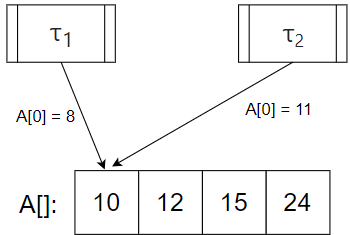
\includegraphics[width=0.4\textwidth]{images/shared_memory.png}
    \caption{An example of two processes writing to a shared in-memory array}
    \label{fig:shared_memory}
\end{figure}
\par
Elixir instead uses a message-passing model for IPC. More specifically, Elixir uses an actor-based model, where each process (actor) has its state and a message box to receive messages from other actors. Actors are responsible for sending a finite number of messages to other actors, spawning new actors and changing their behaviour based on the handling of messages received in the mailbox. Figure \ref{fig:actor_model} shows an example of how actors behave. The mailbox is not necessarily first in, first out (FIFO) but often implementations tend to be.
\begin{figure}[H]
    \centering
    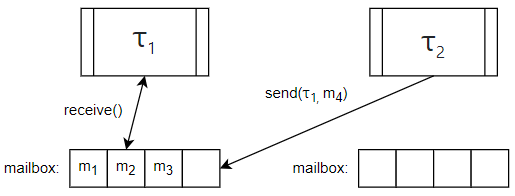
\includegraphics[width=0.6\textwidth]{images/actor_model.png}
    \caption{An example of actors sending and receiving messages under the actor model}
    \label{fig:actor_model}
\end{figure}
\par
In Elixir, a receive statement is used to read messages in the mailbox. The receive block looks through the mailbox for a message that matches a given pattern, if no messages match a given pattern, the process will block until one does.
\begin{lstlisting}[language=Elixir, xleftmargin=.4\linewidth, caption={An example of spawn/1 and spawn/4 in Elixir for spawning a new lightweight process and a new Elixir node}]
    # Example send in Elixir
    send self(), {:hello, "world"}

    # Example receive block in Elixir
    receive do
        {:hello, msg} -> IO.puts msg
    end
\end{lstlisting}
\subsection[]{Quote and Unquote}
The quote and unquote constructs in Elixir give us a deeper insight into how the programming language is implemented. Elixir is fundamentally made of tuples with three elements consisting of an atom\footnote{In Elixir, atoms are named constants, whose values are their own name. They can be identified by a preceding colon, for example, \texttt{:hello}.} that identifies the tuple, an array of metadata and finally the data. For example, the function call \texttt{sum(1, 2)} would be represented by the tuple \texttt{(:sum, [], [1, 2])} and similarly, the variable \texttt{total} would be represented by the tuple \texttt{(:total, [], Elixir)}. Using these building blocks, Elixir can begin to build what is known as a quoted expression, which is a nesting of tuples in a tree-like structure. In many other programming languages, this tree-like structure is referred to as an abstract syntax tree (AST).
\par
The quote and unquote constructs allow us to transition between Elixir syntax and quoted expressions. Using the \texttt{quote/2}\footnote{In Elixir, it is common to name functions or macros alongside their number of arguments. The function \texttt{spawn/1} refers to the function spawn, with 1 argument.} macro on an Elixir block, such as \texttt{quote do: sum(1, 2)} will return the quoted expression representing the block, in this case, \texttt{(:sum, [], [1, 2])}. Similarly, the \texttt{unquote/1} macro can be used within a quoted expression to inject code directly into the underlying expression. Figure \ref{fig:quote_unquote} shows a small example of how unquote can be applied within a quoted expression to inject a variable.
\begin{lstlisting}[language=Elixir, xleftmargin=.4\linewidth, caption={Elixir example of \texttt{quote/2} and \texttt{unquote/1}.}, label={fig:quote_unquote}]
    x = 2
    quote do: sum(1, unquote(x))
\end{lstlisting}
\par

\subsection[]{Metaprogramming}
Metaprogramming is a technique that allows developers to write a program that outputs another program. It means a program can be designed to read or transform other programs. In Elixir, metaprogramming is often used to extend the language by directly modifying the generated quoted expressions by a program. This is achieved through the quote and unquote constructs alongside macros. Macros allow for transforming code and expanding a module.
\par
In Elixir, \texttt{defmacro/2} is used to define new macros, which itself is a macro. Macros receive quoted expressions as arguments and typically inject these expressions into code before returning another quoted expression. Listing \ref{fig:unless} introduces how \texttt{defmacro/2} can be used to define the \texttt{unless/2} macro used in the standard library. Unless is the opposite of an \texttt{if/2} statement, it will execute an expression if a conditional check evaluates to false.
\begin{lstlisting}[language=Elixir, xleftmargin=.3\linewidth, caption={Elixir example of the \texttt{unless/2} macro as defined in the standard library \cite{defmacro}}., label={fig:unless}]
defmacro unless(clause, do: expression) do
  quote do
    if(!unquote(clause), do: unquote(expression))
  end
end
\end{lstlisting}
\par
Macros are both lexical and explicit. That means it is impossible to inject macros globally and it is impossible to run macros without explicit invocation. By leveraging the use of functions, quoted expressions and macros, we can begin to develop a domain-specific language (DSL). For example, constructing a DSL that overrides the standard implementations for many Elixir constructs in a style that makes verifying the correctness of Elixir programs more trivial. By default, Elixir is very difficult to verify. Elixir provides an ExUnit module, with an \texttt{assert/1} macro which could be used for loop invariants, preconditions and postconditions but doesn't support an approach that favours writing verification-aware code. As many Elixir programs are concurrent, and as Elixir uses the actor model, verifying an arbitrary Elixir program that has not been restricted or extended using macros is a challenge.
\par
Another useful feature often associated with the development of DSLs in Elixir is attributes. Attributes can be used to store additional information, as a temporary storage. Attributes also work as constants, or simply to annotate code which can be useful for other developers or the virtual machine. Listing \ref{fig:attributes} shows a basic example of annotating a function with an attribute.
\begin{lstlisting}[language=Elixir, xleftmargin=.3\linewidth, caption={Example use of attributes in Elixir}., label={fig:attributes}]
    @doc "Calculate the sum of two numbers, x and y"
    def sum(x, y) do
        x + y
    end
\end{lstlisting}

\section[]{Existing Work}
\subsection[]{Lean}
\subsection[]{C Wolf}
\subsection[]{Boogie}
\subsection[]{Dafny}
\subsection[]{Promela}
\subsection[]{Gomela}
\section[]{Modelling Elixir Programs in Promela}
\subsection[]{Basic Deadlock}
\subsection[]{Dining Philosophers}
\subsection[]{Preconditions and Postconditions}


\chapter{Veriflixir}
Veriflixir is the main project contribution. The Veriflixir toolchain supports the simulation and verification of a set of Elixir programs. This set is named LTLixir and is detailed in section \ref{sec:ltlixir}. This chapter aims to inform the reader of the constructs defined in LTLixir and how Veriflixir can be used to reason about them. \ref{sec:ltlixir} introduces the LTLixir language and its constructs. \ref{sec:verifiable} provides an example of specifying a verifiable system and how Veriflixir can be used to detect violations of a specification. The subsequent subsections provide further details of more interesting features of LTLixir, such as specifying temporal properties.
\section{LTLixir} \label{sec:ltlixir}
LTLixir is the multi-purpose specification language that compiles to BEAM byte-code and is supported for verification by Veriflixir. Primarily, LTLixir is a subset of Elixir supporting both sequential and concurrent execution. This subset is expressive enough to well-known distributed algorithms such as basic paxos \cite{basic-paxos} and the alternating-bit protocol \cite{ab-protocol}. LTLixir extends Elixir with constructs for specifying temporal properties, specifically LTL properties (where LTLixir derives its name) as well as Floyd-Hoare style logic for specifying pre- and post-conditions. Specifications can be parameterized to identify violations of properties on specific configurations. 
\par

\section{Constructing a Verifiable Elixir Program} \label{sec:verifiable}
This section will walk through the basic construction of an LTLixir program, and show how we can verify the properties of the program using Veriflixir. To begin, we define a server and client process. The server is responsible for creating clients and communicating with them. 
\begin{lstlisting}[language=Elixir, xleftmargin=.3\linewidth, caption={Elixir definition for a server and client module}., label={fig:basic_server}]
    defmodule Server do
        def start_server do
            client = spawn(Client, :start_client, [])
        end
    end

    defmodule Client do
        def start_client do
            IO.puts "Client booted"
        end
    end
\end{lstlisting}
To begin, the server spawns a single client process, which writes to stdio. To ensure correctness when verifying properties of the system, we remove ambiguity by being particular in our naming of the functions \texttt{start\_server} and \texttt{start\_client}. Notice we could name both functions \texttt{start}, but this ambiguity can make it more difficult to digest a trail produced by Veriflixir. With the system implemented, we must now declare an entry point to the system that Veriflixir will use to begin verification. For this example, we can define \texttt{Server.server\_start} as the entry point using an attribute \texttt{\@vae\_init}.

\begin{lstlisting}[language=Elixir, xleftmargin=.3\linewidth, caption={Declaring an entry point to the system}., label={fig:vae_init}]
    @vae_init true
    def start_server do
        client = spawn(Client, :start_client, [])
    end
\end{lstlisting}
Although we set the attribute \texttt{vae\_init} to \texttt{true}, note it is not required that other functions are set to \texttt{false}, this is already implied. With an entry point specified, we can begin using the available tools. By default, Veriflixir reports the presence deadlocks and livelocks in the system. When specifying systems in LTLixir, we do not lose the capability to compile our program to BEAM byte-code, hence the system can still run as a regular Elixir program. For example, using mix \cite{mix}.
\begin{lstlisting}[language=bash, xleftmargin=.3\linewidth]
    $ mix run -e Server.start_server
    Generated app
    Client booted
\end{lstlisting}
More interestingly, we can now use Veriflixir before the Erlang Run-Time System (ERTS) to verify the system adheres to our specification. With no additional properties defined, by running Veriflixir we are ensuring that every possible execution results in a program termination. The presence of a deadlock or livelock will be reported. We can run the Veriflixir executable by passing optional arguments as the path to the specification file. For example, we use the simulator flag $-s$ to run a single simulation of the system.
\begin{lstlisting}[language=bash, xleftmargin=.3\linewidth]
    $ ./veriflixir -s basic_example.ex 
    Client booted
\end{lstlisting}
Alternatively, we can use the $-v$ flag to run the verifier on the specification.
\begin{lstlisting}[language=bash, xleftmargin=.3\linewidth]
    $ ./veriflixir -v basic_example.ex 
    Model checking ran successfully. 0 error(s) found.
    The verifier terminated with no errors.
\end{lstlisting}
\subsection{Detecting a Deadlock} \label{sec:deadlock}
Now we have a basic understanding of what is required to write a specification, we will use Veriflixir to detect a deadlock in the system. By default, the verifier will detect the presence of deadlocks and livelocks in the system. Deadlocks in Elixir programs can be introduced by circular waits, where two simultaneously executing processes are both waiting for a message from the other. To demonstrate this, we modify the existing client and server by introducing a circular wait. The server will now spawn the process, and expect to receive a message from the client, meanwhile, the client will expect to receive a message from the server. The resulting server and client processes are modeled below.
\begin{lstlisting}[language=Elixir, xleftmargin=.3\linewidth, caption={A simple Elixir system with a deadlock}.]
    defmodule Server do
    @vae_init true
    def start_server do
      client = spawn(Client, :start_client, [])
      receive do
        {:im_alive} -> IO.puts "Client is alive"
      end
    end
  end
  
  defmodule Client do
    def start_client do
      receive do
        {:binding} -> IO.puts "Client bound"
      end
    end
  end  
\end{lstlisting}
In this simple example, any execution of the system will result in a deadlock, the system can be considered deterministic in this regard. In many real-world systems with multiple processes, the presence of a deadlock can be difficult to detect due to multiple interleavings. Let's take another look at what happens when we execute the program, run a simulation and run the verifier.
\begin{lstlisting}[language=bash, xleftmargin=.3\linewidth]
$ mix run -e Server.start_server
Generated app
Client booted

\end{lstlisting}
Notice when running the Elixir program, nothing is output to stdio, even though a naive Elixir programmer could think one of the two \texttt{IO.puts} statements is executed. Of course, we know this not to be the case but let's compare the outputs from running Veriflixir.
\begin{lstlisting}[language=bash, xleftmargin=.3\linewidth]
    $ ./veriflixir -s basic_example.ex
    timeout
\end{lstlisting}
The simulator terminates, reporting a timeout. Already, running our specification using Veriflixir provides more information than running the Elixir program. Let's now run the verifier.
\begin{lstlisting}[language=bash, xleftmargin=.2\linewidth]
    $ ./veriflixir -v basic_example.ex
    Model checking ran successfully. 1 error(s) found.
    The program likely reached a deadlock. Generating trace.
    [8] (proc_0) init:4 [receive do]
    [9] (proc_0) init:4 [receive do]
    [10] (proc_0) init:5 [{:im_alive} -> IO.puts "Client is alive"]
    [13] (proc_1) start_client:13 [{:binding} -> IO.puts "Client bound"]
    <<< END OF TRAIL, FINAL STATES: >>>
    [14] (proc_1) start_client:13 [{:binding} -> IO.puts "Client bound"]
    [15] (proc_0) init:5 [{:im_alive} -> IO.puts "Client is alive"]
\end{lstlisting}
Running the verifier produces much more output. Let's break down step by step the output produced by Veriflixir. The first line of the output informs us that the verifier successfully terminated on the input, along with how many errors were found. If an error is found, Veriflixir will use heuristics to profile the type of error, in this case, it has determined the program likely deadlocked. Once determining the error type, an error trail is produced to debug the source of the error. The underlying model derived from the LTLixir specification does not have a one-to-one mapping to the original Elixir code, hence again heuristics are applied to determine where in the Elixir program the trail is produced from. In this case, we can see reference to \texttt{init}, the entry point to the system (annotated previously by \texttt{@vae\_init}). Alongside the process, we can see a line number referring to a line number in the Elixir file, as well as the line of code the line refers to. With the exception of the system entry point, all other function names are labeled as in the original program, for example, $start\_client$. The remaining information on a trail line is less relevant to most users. The first number on a line is the step number (some of these may be omitted for simplicity). The \texttt{proc\_n} refers both to process numbers and function call stack depth.
\par
Now we understand how to read a single line of the trail, we can read the trail in sequential order to learn the interleaving that resulted in the error. In this instance, we can see the server reaches line 5 where it waits for an \texttt{:im\_alive} message from the client and similarly, the client is waiting for a \texttt{:binding} message.
\subsection{Linear Temporal Logic}
We now introduce Linear-time Temporal Logic to our systems to allow us to write more interesting LTLixir specifications. Before doing so, we must detour to type specifications. Type specifications had been previously omitted from examples, but they are imperative for the correctness of LTLixir specifications. LTLixir supports some basic types such as \texttt{integer()}, \texttt{boolean()}, \texttt{atom()} and \texttt{pid()}. Internally, Veriflixir treats process identifiers as integers, so \texttt{integer()} and \texttt{pid()} can be used interchangeably in specifications, for the following examples, we refer to process identifiers as integers. Message passing in specifications should be typed using atoms. To ensure this, any instance of a message should begin with an atom (which we will refer to as the message type). For example, \texttt{{:bind}} and \texttt{{:calculate, 10, 20}} are valid specification messages, \texttt{{false}} would be ignored by Veriflixir. In type specifications, message types are typed as \texttt{atom()}. The atom \texttt{:ok} is reserved to identify non-returning functions. In Elixir, all functions return a value, so in this context, a 'non-returning function' is a function that's value is never matched. We briefly demonstrate the type specifications for two functions, the first is a non-returning function with no arguments and the second function takes two arguments and returns an integer.
\begin{lstlisting}[language=Elixir, xleftmargin=.3\linewidth, caption={Valid type specification examples}.]
    @spec start_server() :: :ok
    def start_server do
        ...
    end

    @spec add(integer(), integer()) :: integer()
    def add a, b do
        ...
    end
\end{lstlisting}
Notice $::$ marks the return type of the function. If these values are matched in the function body, they should not be matched to a different type.
\par
Let's now re-design the server and client processes so we can introduce temporal properties to reason about. The server will now spawn $n$ clients, bind the clients to itself and then await a response from all three clients. To achieve this, we introduce two variables \texttt{client\_n} and \texttt{alive\_clients} that will later be used in our temporal specification.
\begin{lstlisting}[language=Elixir, xleftmargin=.2\linewidth]
    def start_server do
        client_n = 3
        alive_clients = 0
        for _ <- 1..client_n do
            client = spawn(Client, :start_client, [])
            send(client, {:bind, self()})
        end
        alive_clients = check_clients(client_n, alive_clients)
    end
\end{lstlisting}
The implementation of the client process and the \texttt{check\_clients/2} function have been redacted, without understanding their implementation, we can still use our specification to verify the system acts as intended. We introduce our first LTL formula, which verifies that eventually, the number of alive clients is equal to $n$. To introduce an LTL formula, we can use the \texttt{@ltl} attribute. The attribute assigns an LTL formula, as a string, to function. The LTL grammar is defined as the following.
\begin{bnf*}
    \bnfprod{ltl}
      {\bnfpn{operand} \bnfor ( \bnfpn{ltl} ) \bnfor \bnfpn{ltl} \bnfpn{binop} \bnfpn{ltl} \bnfor \bnfpn{unop} \bnfpn{ltl}}\\
    \bnfprod{operand}
      {true \bnfor false \bnfor var \bnfor int \bnfor elixir\_expr}\\
    \bnfprod{unop}
      {\square \bnfor \lozenge \bnfor !}\\
    \bnfprod{binop}
      {U \bnfor W \bnfor V \bnfor \&\& \bnfor || \bnfor \rightarrow \bnfor \leftrightarrow }\\
\end{bnf*}
We want to verify that eventually, the number of alive clients equals the number the server created, we can write this using the formula $\lozenge (alive\_clients \equiv client\_n)$. Using the LTL attribute, we can update our server process.
\begin{lstlisting}[language=Elixir, xleftmargin=.3\linewidth, caption={Example LTL property}.]
    @vae_init true
    @spec start_server() :: :ok
    @ltl "<>(alive_clients == client_n)"
    def start_server do
        ...
    end
\end{lstlisting}
The entire program can be found in appendix \ref{appendix:ex4}. Let us run Veriflixir on the system.
\begin{lstlisting}[language=bash, xleftmargin=.3\linewidth]
    $ ./veriflixir -v basic_example.ex
    Model checking ran successfully. 0 error(s) found.
    The verifier terminated with no errors.
\end{lstlisting}
Let's update the LTL formula, by replacing \texttt{clients\_n} with the number 1 ($\lozenge (alive\_clients \equiv 1)$). We run the verifier again.
\begin{lstlisting}[language=bash, xleftmargin=.1\linewidth]
    $ ./veriflixir -v basic_example.ex
    Model checking ran successfully. 1 error(s) found.
    The program is livelocked, or an ltl property was violated. Generating trace.
\end{lstlisting}
The examples show how LTL properties can be specified and used to verify the system. Given the first LTL property was accepted, we know the formula holds. This is likely because the implementations of the client and \texttt{check\_clients/2} are correct, but we should also specify properties to check the validity of these functions instead of making this assumption.
\par
To help with readability, we can define inline predicates to use in LTL formulae. The predicates that can be defined are formed from a subset of the LTL grammar without the temporal modalities. Inline predicates can refer to variables in the scope of the function. For example, we can define a predicate \( p \) as $alive\_clients \equiv client\_n$. The predicates can take the name of any variable but should not reference variables that are already in scope. To help construct our example, let's also define a predicate \( q \) and set it to \( \neg p \). Using these predicates, we can strengthen our LTL formula to \( (q) \mathcal{U} (\square p) \). Informally, this formula states that there is a moment in time where $alive\_clients \equiv client\_n$, and from that moment onwards this property holds until termination. We can update our \texttt{start\_server} function to reflect this.
\begin{lstlisting}[language=Elixir, xleftmargin=.3\linewidth]
    @ltl "(q)U([]p)"
    def start_server do
      client_n = 3
      alive_clients = 0
      predicate p, alive_clients == client_n
      predicate q, !p
      ...
    end
\end{lstlisting}
\subsection{Pre- and Post-Conditions}
Veriflixir has been designed to target system designs that are bounded in execution. As many real-world systems run long-lived processes, it is important that when writing LTLixir specifications there is a focus on termination conditions. For many distributed algorithms this could be completing a round of communication, reaching a consensus, awaiting a specific message to be received or reaching a stable system state. To aid this, LTLixir supports Floyd-Hoare style pre- and post-conditions in function definitions. These are particularly useful for ensuring proper bounds on the system that help define correct execution. Consider a process that should send and receive a single message each round. We can define a pre-condition on a bounded parameter to ensure the process does not run indefinitely. Let us refactor the client process to complete a number of rounds (determined by the server) before terminating. The client will receive a \texttt{:bind} message from the server, deciding how many rounds to complete and then will recurse until it has completed all the rounds.
\begin{lstlisting}[language=Elixir, xleftmargin=.3\linewidth]
    defmodule Client do
        @spec start_client() :: :ok
        def start_client do
            {server, rounds} = receive do
            {:bind, sender, round_limit} -> {sender, round_limit}
            end
            next_round(server, rounds)
        end

        @spec next_round(pid(), integer()) :: :ok
        def next_round(server, rounds) do
            send(server, {:im_alive})
            next_round(server, rounds - 1)
        end
    end
\end{lstlisting}
We can again run this with mix, and we can observe that the server terminates. Although our clients did not terminate, there was no indication of this. Processes in Elixir are isolated, so the termination of the server does not imply the termination of the clients (links can resolve this \cite{elixir_links}). It has become challenging to determine if our client is truely behaving as intended.
\begin{lstlisting}[language=bash, xleftmargin=.3\linewidth]
    $ mix run -e Server.start_server
    Generated app
    $
\end{lstlisting}
To help reason about this, we introduce the \texttt{defv} macro from the LTLixir specification language. The \texttt{defv} macro is used to define pre- and post-conditions on functions. Pre-conditions check conditions regarding the values of function arguments on entry to the function and similarly, post-conditions can assert conditions on values within the scope of the function on exit. For example, we could define a function \texttt{add\_positives/2} that takes two strictly positive numbers and sums them.
\begin{lstlisting}[language=Elixir, xleftmargin=.0\linewidth, caption={Example usage of pre- and post-conditions in LTLixir}]
    defv add_positives(a, b), pre: a > 0 and b > 0, post: result == a + b do
        ...
    end
\end{lstlisting}
With this definition, we gain assurances that the implementation of the function behaves as we expect and that no other function interacts with the function in a manner that violates our expected behavior. Let's take a similar approach with our client to help understand why the program does not terminate.
\begin{lstlisting}[language=Elixir, xleftmargin=.3\linewidth]
    @spec next_round(pid(), integer()) :: :ok
    defv next_round(server, rounds), pre: rounds >= 0 do
        ...
    end
\end{lstlisting}
We can run Veriflixir on the system to verify the pre-condition holds for every possible execution.
\begin{lstlisting}[language=bash, xleftmargin=.1\linewidth]
    $ ./veriflixir -v basic_example.ex
    Model checking ran successfully. 1 error(s) found.
    An LTL, pre- or post-condition was violated. Generating trace.
    Violated: assertion violated (rounds>=0) (at depth 45).
\end{lstlisting}
Veriflixir reports an error, in particular, it notes the violation of an assertion. An assertion violation can be a violation of an LTL formula, and pre-condition or a post-condition. In this case, it outputs the assertion that was violated \texttt{rounds >= 0}, which we are aware is our pre-condition. The depth refers to how many transitions were taken in the execution path before violation, to most users this information is not useful.
\subsection{Parameterized Systems}
Up to this point, we have declared various system properties such as \texttt{client\_n}, \texttt{alive\_client} and \texttt{rounds}. In reality, the value assigned to these properties could be determined by many factors and it may not be known to the developer at the time of writing the specification. To support this, LTLixir allows us to declare these properties as parameters, in particular, we want to declare concurrency parameters. We define concurrency parameters are variables that impact the behaviour of a distributed system (we will simply refer to them as parameters going forward). For example, in a consensus algorithm such as paxos, we may have variables to determine the number of acceptors, proposers and size of a quorum. We can declare these variables as parameters in the specification in order to verify the system for multiple possible configurations. Typically, the values used in these auto-generated configurations will be small values as large values may lead to a state-space that becomes difficult to explore.
\par
To mark a variable as a parameter, we again make use of attributes. The \texttt{@params} attribute takes a tuple of atoms referencing variables in the function scope. For example, \texttt{@params {:x, :y}} declares that $x$ and $y$ are configurable parameters that the verifier will explore. We can apply this definition to our existing server process.
\begin{lstlisting}[language=Elixir, xleftmargin=.3\linewidth, caption={Example of declaring concurrency parameters in specification.}]
    @params {:client_n, :number_of_rounds}
    def start_server do
      client_n = 3
      number_of_rounds = 2
      predicate p, alive_clients == client_n * number_of_rounds
      ...
    end
\end{lstlisting}
We can declare as many parameters as required. The values matched in the declaration of the variables will be ignored if we run Veriflixir in parameterized mode. To run the verifier, we can use the $-p$ flag. The verifier will calculate an acceptance confidence, \(\alpha \in [0, 1]\), where an $\alpha$ of 1 indicates all configurations were accepted by the verifier and an $\alpha$ of 0 indicates no configurations were accepted. In the case $\alpha < 1$, the verifier will output configurations that lead to violations in the system. Then, the system can run in verification mode to reproduce a trail that results in the violation. To run the parameterized verification, we use the same command but with the $-p$ flag.
\begin{lstlisting}[language=bash, xleftmargin=.1\linewidth]
    $ ./veriflixir -p basic_example.ex 
    Generating models.
    Generated 9 models.
    Acceptance confidence: 1.
\end{lstlisting}
We can introduce a bug into our program that will cause a violation of the specification to show the output of the verifier under these circumstances. To introduce a bug, we are going to conditionally call \texttt{check\_clients/2} if \texttt{client\_n > 1} holds.
\begin{lstlisting}[language=Elixir, xleftmargin=.1\linewidth]
@params {:number_of_rounds}
def start_server do
    ...
    alive_clients = if number_of_rounds > 1 do
        check_clients(client_n * number_of_rounds, alive_clients)
    else
        0
    end
end
\end{lstlisting}
This will now result in cases where the temporal property is violated, as $\texttt{alive\_clients} \equiv \texttt{client\_n} * \texttt{number\_of\_rounds}$ will not hold for all configurations. Note that we have reduced the parameters down to just \texttt{\{number\_of\_rounds\}}. The system is theoretically capable of handling any number of parameters in its search, however the computational cost of exploring the state-space grows exponentially with the number of parameters, hence in reality we should use our understanding of the system to determine which parameters to test at a time.
\begin{lstlisting}[language=bash, xleftmargin=.1\linewidth]
$ ./veriflixir -p 3 basic_example.ex`
Generating models.
Generated 3 models.
Acceptance confidence: 0.6666666666666667.
Violations found in models:
Model with params: {"number_of_rounds": '1'}
Assign these parameters to the system and re-run the verifier in verification mode to gather a trace.
\end{lstlisting}
The system found a violation for the assignment of 1 to \texttt{number\_of\_rounds}. To investigate, we could run the verifier using the $-v$ flag on this configuration. We also now see our acceptance confidence has dropped below 1, due to an error produced by one of the configurations. It's also useful to note that Veriflixir was executed with $-p 3$, this sets the range of values for the parameter, large numbers are not recommended and most users will find 3 sufficient. 
\section{Summary}
We have now given a high-level overview of Veriflixir, the verification toolchain capable of verifying Elixir programs written using the LTLixir specification. We saw how to use Veriflixir to simulate executions of the system, verify our system's adherence to a specification and parameterize concurrency parameters for exploration. This chapter also exposed how to use LTLixir constructs to reason about temporal properties as well as how pre- and post-conditions can drive functional correctness. The next chapter will begin to explore the implementation behind Veriflixir.
\chapter{Evaluation}
In this chapter, we aim to evaluate the expressiveness of Veriflixir's design. First, we perform a quantitive analysis of modeling classical distributed algorithms such as basic paxos in section \ref{sec:paxos} and the alternating-bit protocol in section \ref{sec:ab}. Section \ref{sec:vs} will delve into a comparison against current state-of-the art model checking techniques for modern day programming languages. Finally, we will explore the performance of Veriflixir in a growing sytem in section \ref{sec:perf}.
\section{Analysing Distributed Systems}
Verifying the correctness of real-world distributed systems is a major motivation for this project. Critical real-time systems (such as in air-traffic control or healthcare  \cite{airlines,healthcare}) should not fail and should rely on rigerous verification techniques to guarantee production code is correct.  
\subsection{Basic Paxos} \label{sec:paxos}
Paxos is an example of a distributed algorithm \cite{paxos_simple}. It is a consensus algorithm, where many processes are tasked to agree on a value. Processes may propose what this value should be, but only one value should be agreed upon. The safety requirements for consensus are:
\begin{itemize}
    \item Only a value that has been proposed may be chosen.
    \item Only a single value is chosen.
    \item A process never learns that a value has been chosen unless it actually has.
\end{itemize}
The system's liveness requirement is that a proposed value is eventually chosen and if a value if chosen then a process can learn the chosen value.
\subsubsection{Informal Specification}
There are many flavors to the paxos algorithm. We will informally present a basic, one-shot paxos. 
\subsubsection{Comparison with 'Model Checking Paxos in Spin' Paper}
\subsection{Alternating-bit Protocol} \label{sec:ab}
\subsubsection{Informal Specification}
\subsubsection{Experimental Analysis}
\section{Veriflixir vs } \label{sec:vs}
\section{Performance} \label{sec:perf}
\chapter{Conclusion}
In this paper, we aimed to provide modelling and verification techniques for message-passing systems. To evaluate these techniques, we targetted Elixir, the actor-based, concurrent programming language. As part of our research, we introduced Verlixir, a verification-aware language for message-passing systems.
\\ \\
This project aimed to achieve some key objectives required for specifying and implementing distributed algorithms in a `correct' manner. The specification language supported by Verlixir, alongside Verlixir's operational modes, moves towards achieving these objectives.
\\ \\
Verlixir provides a simulator capable of simulating large-scale distributed systems. These systems can be implemented in a modern programming language, and simulated in a controlled environment. This allows developers to prototype complex systems and observe their behaviour before deploying them in a production environment. Because Verlixir directly integrates with Elixir, the system can be easily transferred from simulation to production.
\\ \\
We also have empowered developers to verify the behaviour of systems, ensuring formal safety and liveness properties are adhered to. These properties can be specified alongside the implementation of the system, and verified without the need for a separate model. Counterexamples are produced in an Elixir-friendly format, allowing developer to debug the system and understand why a property was violated; particularly focusing on the message-passing interleaving that caused the violation.
\\ \\
To extend confidence, Verlixir supports modelling systems across different configurations. This ensures systems behave consistently across different environments. This is particularly useful for distributed systems that are subject to network partitions, or systems that are required to scale up or down.
\section{Future Work}
Throughout the course of research, we have identified several areas for future work. We have indicated some of these areas previously, but we will discuss them in more detail here. An obvious extension would involve supporting a larger Elixir feature set, but we will go into depth on more unique extensions.
\\ \\
A large inspiration for this project was the verification-aware language, Dafny. The Dafny language sets out to achieve similar claims to Verlixir, but takes a different approach. Dafny fundamentally relies on theorem proving for verification, whereas Verlixir uses model checking. In particular, Dafny transpiles to Boogie, a verification-aware intermediate language. Boogie currently then uses Z3 for theorem proving. Theorem proving provides formal proofs of correctness, which give stronger claims than the pre- and post-condition checks we assert in model checking. We believe an ideal solution to verify message-passing systems could involve a combination of both theorem proving and model checking. We could extend Verlixir to support theorem proving within Elixir processes, and then continue to use model checking for verifying inter-process communication. This would provide a stronger guarantee of correctness for the system as a whole.
\\ \\
We explored the differences between Verlixir and other verification-aware languages. A key insight we drew from this is the lack of capability for injecting faults into models. Many distributed algorithms have been designed with an approach such that given there are no more than $n$ faults, the system will still follow the specification. In order to truly scrutinise these algorithms, we need the capability to inject faults into the system. A simple extension to Verlixir could involve injecting random terminating faults into processes, and then observing the system's fault tolerance under these conditions.
\\ \\
A second insight gathered from comparing tools is the lack of support for verifying computation tree logic (CTL) in modern programming languages. CTL is a temporal logic that allows us to reason about paths in a system. A simple example of where CTL could be useful is in verifying the Paxos algorithm. To ensure fairness between all proposers, we could specify and verify a CTL property that states: there exists a path where each proposal is accepted. We believe that extending Verlixir to support CTL would provide a more comprehensive verification framework for message-passing systems.
\section{Ethical Considerations}
Throughout the report we make reference to critical distributed-systems used in the contexts of air traffic control and healthcare. While the tools and research discussed are designed to improve the reliability of these systems, relying on them in isolation is not sufficient. Testing distributed systems is hard, and it is important that rigorous testing is performed by multiple parties using multiple techniques. That said, we believe Verlixir provides an advancement in the verification of distributed systems.
\section{Final Remarks}
The goal for this project was to design a tool that could verify real-world distributed algorithms which are used in research and industry. Throughout researching Verlixir, many notional examples were used to demonstrate the capabilities of the tool. Through the evaluation, we have shown these capabilities extend to real, well-known algorithms such as Paxos and Raft. In achieving this, we believe Verlixir has the potential to be a valuable tool for verifying distributed systems.
\\ \\
Historically, model checking has required hand-translation of code into a model. Verlixir lowers the barrier to entry for verifying systems. If a programmer can write their implementation using the provided LTLixir set, the system verification comes for free. We believe moving towards a world where verification-aware languages become the standard, will greatly improve the reliability of code. Instead of programmers thinking about how to implement a system, they can focus on what the system should do. A shift in mindset away from implementation specifics, towards reasoning about the safety and liveness of a system means that we can describe our systems in a more holistic way.
\\ \\
With the recent rise in artificially intelligent copilots \cite{attention_is, copilot_asset,safety_ai}, the future of programming could move towards a more declarative style. We programmers, could simply be burdened to write the system specification, in terms of safety and liveness, and a large-language model could generate the implementation.
\appendix
\chapter{First Appendix}
\section{Verlixir Example}

\begin{lstlisting}[language=Elixir, xleftmargin=.1\linewidth]
  import VaeLib

  defmodule Server do
    @vae_init true
    @ltl "(q)U([]p)"
    @spec start_server() :: :ok
    @params {:number_of_rounds}
    def start_server do
      predicate p, alive_clients == client_n * number_of_rounds
      predicate q, !p
      client_n = 1
      number_of_rounds = 2
      alive_clients = 0
      for _ <- 1..client_n do
        client = spawn(Client, :start_client, [])
        send(client, {:bind, self(), number_of_rounds})
      end
      alive_clients = if number_of_rounds > 1 do
        check_clients(client_n * number_of_rounds, alive_clients)
      else
        0
      end
    end
  
    @spec check_clients(integer(), integer()) :: integer()
    def check_clients(expected_clients, current_clients) do
      if expected_clients == current_clients do
        current_clients
      else
        receive do
          {:im_alive} -> check_clients(expected_clients, current_clients + 1)
        end
      end
    end
  end
  
  defmodule Client do
    @spec start_client() :: :ok
    def start_client do
      {server, rounds} = receive do
        {:bind, sender, round_limit} -> {sender, round_limit}
      end
      next_round(server, rounds)
    end
  
    @spec next_round(pid(), integer()) :: :ok
    defv next_round(server, rounds), pre: rounds >= 0 do
      if rounds == 0 do
        :ok
      else
        send(server, {:im_alive})
        next_round(server, rounds - 1)
      end
    end
  end
  
\end{lstlisting}

\section{Paxos}
\subsubsection{First paxos implementation with a bug}
\begin{lstlisting}[language=Elixir, xleftmargin=.1\linewidth]
import VaeLib

defmodule Acceptor do

  @spec start_acceptor() :: :ok
  def start_acceptor do
    acceptedProposal = -1
    acceptedValue = -1
    minProposal = -1
    accept_handler(acceptedProposal, acceptedValue, minProposal)
  end

  @spec accept_handler(integer(), integer(), integer()) :: :ok
  def accept_handler(acceptedProposal, acceptedValue, minProposal) do
    receive do
      {:prepare, n, proposer} ->
        if n > minProposal do
          send proposer, {:promise, acceptedProposal, acceptedValue}
          accept_handler(acceptedProposal, acceptedValue, n)
        else
          send proposer, {:promise, acceptedProposal, acceptedValue}
          accept_handler(acceptedProposal, acceptedValue, minProposal)
        end
      {:accept, n, value, proposer} ->
        if n >= minProposal do
          send proposer, {:accepted, n}
          accept_handler(n, value, n)
        else
          send proposer, {:accepted, minProposal}
          accept_handler(acceptedProposal, acceptedValue, minProposal)
        end
      {:terminate} ->
        IO.puts("Terminating acceptor")
    end
  end
end

defmodule Proposer do
  @spec start_proposer() :: :ok
  def start_proposer do
    receive do
      {:bind, acceptors, proposal_n, value, maj, learner} -> proposer_handler(acceptors, proposal_n, value, maj, learner)
    end
  end

  @spec proposer_handler(list(), integer(), integer(), integer(), integer()) :: :ok
  def proposer_handler(acceptors, proposal_n, value, maj, learner) do
    for acceptor <- acceptors do
      send acceptor, {:prepare, proposal_n, self()}
    end

    receive_prepared(proposal_n, value, maj, 0, 0)
    {prepared_n, prepared_value} = receive do
      {:majority_prepared, n, v} -> {n, v}
    end

    for acceptor <- acceptors do
      send acceptor, {:accept, prepared_n, prepared_value, self()}
    end

    accepted_n = receive_accepted(maj, prepared_n, 0, 0)

    if accepted_n != -1 do
      # Value chosen
      send learner, {:learned, prepared_value}
    else
      # Value was rejected
      send learner, {:learned, 0}
    end
  end

  @spec receive_prepared(integer(), integer(), integer(), integer(), integer()) :: :ok
  def receive_prepared(proposal_n, value, maj, highest_seen_proposal, count) do
    if count >= maj do
      send self(), {:majority_prepared, proposal_n, value}
    else
      receive do
        {:promise, acceptedProposal, acceptedValue} ->
          if acceptedValue != -1 && acceptedProposal > highest_seen_proposal do
            receive_prepared(proposal_n, acceptedValue, maj, acceptedProposal, count + 1)
          else
            receive_prepared(proposal_n, value, maj, highest_seen_proposal, count + 1)
          end
      end
    end
  end

  @spec receive_accepted(integer(), integer(), integer(), integer()) :: integer()
  def receive_accepted(maj, prepared_n, rejections, count) do
    if count >= maj do
      if rejections >= maj do  # BUG IS HERE
        -1
      else
        prepared_n
      end
    else
      receive do
        {:accepted, n} ->
          if n > prepared_n do
            receive_accepted(maj, prepared_n, rejections + 1, count + 1)
          else
            receive_accepted(maj, prepared_n, rejections, count + 1)
          end
      end
    end
  end
end

defmodule Learner do

  @spec start() :: :ok
  @vae_init true
  def start do
    n_acceptors = 3
    quorum = 2
    n_proposers = 2
    vals = [42, 31]
    acceptors = for _ <- 1..n_acceptors do
      spawn(Acceptor, :start_acceptor, [])
    end

    for i <- 1..n_proposers do
      proposer = spawn(Proposer, :start_proposer, [])
      val_i = i - 1
      val = Enum.at(vals, val_i)
      send proposer, {:bind, acceptors, i, val, quorum, self()}
    end
    wait_learned(acceptors, n_proposers, 0)
  end

  @spec wait_learned(list(), integer(), integer()) :: :ok
  @ltl """
  []((p->!<>q) && (q->!<>p))
  <>(r)
  [](s)
  """
  def wait_learned(acceptors, p_n, learned_n) do
    predicate p, final_value == 31
    predicate q, final_value == 42
    predicate r, final_value != 0
    predicate s, final_value == 0 || final_value == 31 || final_value == 42

    if p_n == learned_n do
      for acceptor <- acceptors do
        send acceptor, {:terminate}
      end
    else
      receive do
        {:learned, final_value} ->
          IO.puts("Learned final_value:")
          IO.puts(final_value)
      end
      wait_learned(acceptors, p_n, learned_n + 1)
    end
  end
end

\end{lstlisting}

\subsubsection{First paxos bug message log}
\begin{lstlisting}[xleftmargin=.01\linewidth, xrightmargin=0.01\linewidth, caption={Message passing caused by the proposer's protocol bug.}, label={lst:paxos_bug}]
    Never claim moves to line 6     [(1)]
138:    proc  7 (start_proposer:1) test_out.pml:314 Recv 7,BIND,0,0,2,0,0,0,0,0,1,0,0,0,0,0,42,0,0,0,0,0,2,0,0,0,0,0,0,0,0,0,0,0,0,0,0,0        <- queue 20 (__BIND)
154:    proc  8 (proposer_handler:1) test_out.pml:350 Send 1,PREPARE,0,0,1,0,0,0,0,0,7,0,0,0,0,0,0,0,0,0,0,0,0,0,0,0,0,0,0,0,0,0,0,0,0,0,0,0    -> queue 23 (__PREPARE)
158:    proc  8 (proposer_handler:1) test_out.pml:350 Send 3,PREPARE,0,0,1,0,0,0,0,0,7,0,0,0,0,0,0,0,0,0,0,0,0,0,0,0,0,0,0,0,0,0,0,0,0,0,0,0    -> queue 23 (__PREPARE)
162:    proc  8 (proposer_handler:1) test_out.pml:350 Send 5,PREPARE,0,0,1,0,0,0,0,0,7,0,0,0,0,0,0,0,0,0,0,0,0,0,0,0,0,0,0,0,0,0,0,0,0,0,0,0    -> queue 23 (__PREPARE)
197:    proc  6 (accept_handler:1) test_out.pml:262 Recv 5,PREPARE,0,0,1,0,0,0,0,0,7,0,0,0,0,0,0,0,0,0,0,0,0,0,0,0,0,0,0,0,0,0,0,0,0,0,0,0      <- queue 23 (__PREPARE)
203:    proc  6 (accept_handler:1) test_out.pml:272 Send 7,PROMISE,0,0,-1,0,0,0,0,0,-1,0,0,0,0,0,0,0,0,0,0,0,0,0,0,0,0,0,0,0,0,0,0,0,0,0,0,0    -> queue 26 (__PROMISE)
205:    proc  9 (receive_prepared:1) test_out.pml:425 Recv 7,PROMISE,0,0,-1,0,0,0,0,0,-1,0,0,0,0,0,0,0,0,0,0,0,0,0,0,0,0,0,0,0,0,0,0,0,0,0,0,0  <- queue 26 (__PROMISE)
219:    proc  2 (accept_handler:1) test_out.pml:262 Recv 1,PREPARE,0,0,1,0,0,0,0,0,7,0,0,0,0,0,0,0,0,0,0,0,0,0,0,0,0,0,0,0,0,0,0,0,0,0,0,0      <- queue 23 (__PREPARE)
262:    proc  4 (accept_handler:1) test_out.pml:262 Recv 3,PREPARE,0,0,1,0,0,0,0,0,7,0,0,0,0,0,0,0,0,0,0,0,0,0,0,0,0,0,0,0,0,0,0,0,0,0,0,0      <- queue 23 (__PREPARE)
278:    proc  0 (:init::1) test_out.pml:521 Send 10,BIND,0,0,3,0,0,0,0,0,2,0,0,0,0,0,31,0,0,0,0,0,2,0,0,0,0,0,0,0,0,0,0,0,0,0,0,0       -> queue 20 (__BIND)
292:    proc  4 (accept_handler:1) test_out.pml:272 Send 7,PROMISE,0,0,-1,0,0,0,0,0,-1,0,0,0,0,0,0,0,0,0,0,0,0,0,0,0,0,0,0,0,0,0,0,0,0,0,0,0    -> queue 26 (__PROMISE)
300:    proc 11 (receive_prepared:1) test_out.pml:425 Recv 7,PROMISE,0,0,-1,0,0,0,0,0,-1,0,0,0,0,0,0,0,0,0,0,0,0,0,0,0,0,0,0,0,0,0,0,0,0,0,0,0  <- queue 26 (__PROMISE)
344:    proc  2 (accept_handler:1) test_out.pml:272 Send 7,PROMISE,0,0,-1,0,0,0,0,0,-1,0,0,0,0,0,0,0,0,0,0,0,0,0,0,0,0,0,0,0,0,0,0,0,0,0,0,0    -> queue 26 (__PROMISE)
346:    proc 10 (start_proposer:1) test_out.pml:314 Recv 10,BIND,0,0,3,0,0,0,0,0,2,0,0,0,0,0,31,0,0,0,0,0,2,0,0,0,0,0,0,0,0,0,0,0,0,0,0,0       <- queue 20 (__BIND)
370:    proc 14 (receive_prepared:1) test_out.pml:421 Send 7,MAJORITY_PREPARED,0,0,1,0,0,0,0,0,42,0,0,0,0,0,0,0,0,0,0,0,0,0,0,0,0,0,0,0,0,0,0,0,0,0,0,0 -> queue 46 (__MAJORITY_PREPARED)
372:    proc  8 (proposer_handler:1) test_out.pml:363 Recv 7,MAJORITY_PREPARED,0,0,1,0,0,0,0,0,42,0,0,0,0,0,0,0,0,0,0,0,0,0,0,0,0,0,0,0,0,0,0,0,0,0,0,0 <- queue 46 (__MAJORITY_PREPARED)
382:    proc  8 (proposer_handler:1) test_out.pml:386 Send 1,ACCEPT,0,0,1,0,0,0,0,0,42,0,0,0,0,0,7,0,0,0,0,0,0,0,0,0,0,0,0,0,0,0,0,0,0,0,0,0    -> queue 47 (__ACCEPT)
386:    proc  8 (proposer_handler:1) test_out.pml:386 Send 3,ACCEPT,0,0,1,0,0,0,0,0,42,0,0,0,0,0,7,0,0,0,0,0,0,0,0,0,0,0,0,0,0,0,0,0,0,0,0,0    -> queue 47 (__ACCEPT)
390:    proc  8 (proposer_handler:1) test_out.pml:386 Send 5,ACCEPT,0,0,1,0,0,0,0,0,42,0,0,0,0,0,7,0,0,0,0,0,0,0,0,0,0,0,0,0,0,0,0,0,0,0,0,0    -> queue 47 (__ACCEPT)
421:    proc 15 (proposer_handler:1) test_out.pml:350 Send 1,PREPARE,0,0,2,0,0,0,0,0,10,0,0,0,0,0,0,0,0,0,0,0,0,0,0,0,0,0,0,0,0,0,0,0,0,0,0,0   -> queue 23 (__PREPARE)
425:    proc 15 (proposer_handler:1) test_out.pml:350 Send 3,PREPARE,0,0,2,0,0,0,0,0,10,0,0,0,0,0,0,0,0,0,0,0,0,0,0,0,0,0,0,0,0,0,0,0,0,0,0,0   -> queue 23 (__PREPARE)
429:    proc 15 (proposer_handler:1) test_out.pml:350 Send 5,PREPARE,0,0,2,0,0,0,0,0,10,0,0,0,0,0,0,0,0,0,0,0,0,0,0,0,0,0,0,0,0,0,0,0,0,0,0,0   -> queue 23 (__PREPARE)
452:    proc 16 (accept_handler:1) test_out.pml:262 Recv 1,PREPARE,0,0,2,0,0,0,0,0,10,0,0,0,0,0,0,0,0,0,0,0,0,0,0,0,0,0,0,0,0,0,0,0,0,0,0,0     <- queue 23 (__PREPARE)
458:    proc 16 (accept_handler:1) test_out.pml:272 Send 10,PROMISE,0,0,-1,0,0,0,0,0,-1,0,0,0,0,0,0,0,0,0,0,0,0,0,0,0,0,0,0,0,0,0,0,0,0,0,0,0   -> queue 26 (__PROMISE)
460:    proc 12 (accept_handler:1) test_out.pml:282 Recv 5,ACCEPT,0,0,1,0,0,0,0,0,42,0,0,0,0,0,7,0,0,0,0,0,0,0,0,0,0,0,0,0,0,0,0,0,0,0,0,0      <- queue 47 (__ACCEPT)
466:    proc 12 (accept_handler:1) test_out.pml:291 Send 7,ACCEPTED,0,0,1,0,0,0,0,0,0,0,0,0,0,0,0,0,0,0,0,0,0,0,0,0,0,0,0,0,0,0,0,0,0,0,0,0     -> queue 48 (__ACCEPTED)
474:    proc 17 (accept_handler:1) test_out.pml:282 Recv 1,ACCEPT,0,0,1,0,0,0,0,0,42,0,0,0,0,0,7,0,0,0,0,0,0,0,0,0,0,0,0,0,0,0,0,0,0,0,0,0      <- queue 47 (__ACCEPT)
492:    proc 17 (accept_handler:1) test_out.pml:296 Send 7,ACCEPTED,0,0,2,0,0,0,0,0,0,0,0,0,0,0,0,0,0,0,0,0,0,0,0,0,0,0,0,0,0,0,0,0,0,0,0,0     -> queue 48 (__ACCEPTED)
494:    proc 13 (accept_handler:1) test_out.pml:262 Recv 3,PREPARE,0,0,2,0,0,0,0,0,10,0,0,0,0,0,0,0,0,0,0,0,0,0,0,0,0,0,0,0,0,0,0,0,0,0,0,0     <- queue 23 (__PREPARE)
500:    proc 13 (accept_handler:1) test_out.pml:272 Send 10,PROMISE,0,0,-1,0,0,0,0,0,-1,0,0,0,0,0,0,0,0,0,0,0,0,0,0,0,0,0,0,0,0,0,0,0,0,0,0,0   -> queue 26 (__PROMISE)
512:    proc 18 (receive_accepted:1) test_out.pml:459 Recv 7,ACCEPTED,0,0,1,0,0,0,0,0,0,0,0,0,0,0,0,0,0,0,0,0,0,0,0,0,0,0,0,0,0,0,0,0,0,0,0,0   <- queue 48 (__ACCEPTED)
542:    proc 21 (accept_handler:1) test_out.pml:262 Recv 5,PREPARE,0,0,2,0,0,0,0,0,10,0,0,0,0,0,0,0,0,0,0,0,0,0,0,0,0,0,0,0,0,0,0,0,0,0,0,0     <- queue 23 (__PREPARE)
554:    proc 20 (receive_prepared:1) test_out.pml:425 Recv 10,PROMISE,0,0,-1,0,0,0,0,0,-1,0,0,0,0,0,0,0,0,0,0,0,0,0,0,0,0,0,0,0,0,0,0,0,0,0,0,0 <- queue 26 (__PROMISE)
560:    proc 23 (accept_handler:1) test_out.pml:282 Recv 3,ACCEPT,0,0,1,0,0,0,0,0,42,0,0,0,0,0,7,0,0,0,0,0,0,0,0,0,0,0,0,0,0,0,0,0,0,0,0,0      <- queue 47 (__ACCEPT)
578:    proc 23 (accept_handler:1) test_out.pml:296 Send 7,ACCEPTED,0,0,2,0,0,0,0,0,0,0,0,0,0,0,0,0,0,0,0,0,0,0,0,0,0,0,0,0,0,0,0,0,0,0,0,0     -> queue 48 (__ACCEPTED)
580:    proc 21 (accept_handler:1) test_out.pml:272 Send 10,PROMISE,0,0,1,0,0,0,0,0,42,0,0,0,0,0,0,0,0,0,0,0,0,0,0,0,0,0,0,0,0,0,0,0,0,0,0,0    -> queue 26 (__PROMISE)
582:    proc 24 (receive_prepared:1) test_out.pml:425 Recv 10,PROMISE,0,0,-1,0,0,0,0,0,-1,0,0,0,0,0,0,0,0,0,0,0,0,0,0,0,0,0,0,0,0,0,0,0,0,0,0,0 <- queue 26 (__PROMISE)
602:    proc 25 (receive_prepared:1) test_out.pml:421 Send 10,MAJORITY_PREPARED,0,0,2,0,0,0,0,0,31,0,0,0,0,0,0,0,0,0,0,0,0,0,0,0,0,0,0,0,0,0,0,0,0,0,0,0        -> queue 46 (__MAJORITY_PREPARED)
616:    proc 15 (proposer_handler:1) test_out.pml:363 Recv 10,MAJORITY_PREPARED,0,0,2,0,0,0,0,0,31,0,0,0,0,0,0,0,0,0,0,0,0,0,0,0,0,0,0,0,0,0,0,0,0,0,0,0        <- queue 46 (__MAJORITY_PREPARED)
626:    proc 15 (proposer_handler:1) test_out.pml:386 Send 1,ACCEPT,0,0,2,0,0,0,0,0,31,0,0,0,0,0,10,0,0,0,0,0,0,0,0,0,0,0,0,0,0,0,0,0,0,0,0,0   -> queue 47 (__ACCEPT)
630:    proc 15 (proposer_handler:1) test_out.pml:386 Send 3,ACCEPT,0,0,2,0,0,0,0,0,31,0,0,0,0,0,10,0,0,0,0,0,0,0,0,0,0,0,0,0,0,0,0,0,0,0,0,0   -> queue 47 (__ACCEPT)
634:    proc 15 (proposer_handler:1) test_out.pml:386 Send 5,ACCEPT,0,0,2,0,0,0,0,0,31,0,0,0,0,0,10,0,0,0,0,0,0,0,0,0,0,0,0,0,0,0,0,0,0,0,0,0   -> queue 47 (__ACCEPT)
659:    proc 27 (receive_accepted:1) test_out.pml:459 Recv 7,ACCEPTED,0,0,2,0,0,0,0,0,0,0,0,0,0,0,0,0,0,0,0,0,0,0,0,0,0,0,0,0,0,0,0,0,0,0,0,0   <- queue 48 (__ACCEPTED)
681:    proc 29 (accept_handler:1) test_out.pml:282 Recv 5,ACCEPT,0,0,2,0,0,0,0,0,31,0,0,0,0,0,10,0,0,0,0,0,0,0,0,0,0,0,0,0,0,0,0,0,0,0,0,0     <- queue 47 (__ACCEPT)
699:    proc 29 (accept_handler:1) test_out.pml:291 Send 10,ACCEPTED,0,0,2,0,0,0,0,0,0,0,0,0,0,0,0,0,0,0,0,0,0,0,0,0,0,0,0,0,0,0,0,0,0,0,0,0    -> queue 48 (__ACCEPTED)
701:    proc 28 (receive_accepted:1) test_out.pml:459 Recv 10,ACCEPTED,0,0,2,0,0,0,0,0,0,0,0,0,0,0,0,0,0,0,0,0,0,0,0,0,0,0,0,0,0,0,0,0,0,0,0,0  <- queue 48 (__ACCEPTED)
707:    proc 30 (receive_accepted:1) test_out.pml:454 Send 1    -> queue 78 (ret)
711:    proc 22 (accept_handler:1) test_out.pml:282 Recv 1,ACCEPT,0,0,2,0,0,0,0,0,31,0,0,0,0,0,10,0,0,0,0,0,0,0,0,0,0,0,0,0,0,0,0,0,0,0,0,0     <- queue 47 (__ACCEPT)
717:    proc 27 (receive_accepted:1) test_out.pml:466 Recv 1    <- queue 78 (ret1)
719:    proc 27 (receive_accepted:1) test_out.pml:467 Send 1    -> queue 54 (ret)
721:    proc 18 (receive_accepted:1) test_out.pml:471 Recv 1    <- queue 54 (ret2)
723:    proc 18 (receive_accepted:1) test_out.pml:472 Sent 1    -> queue 22 (ret)
724:    proc  8 (proposer_handler:1) test_out.pml:396 Recv 1    <- queue 22 (ret2)
740:    proc 22 (accept_handler:1) test_out.pml:291 Send 10,ACCEPTED,0,0,2,0,0,0,0,0,0,0,0,0,0,0,0,0,0,0,0,0,0,0,0,0,0,0,0,0,0,0,0,0,0,0,0,0    -> queue 48 (__ACCEPTED)
742:    proc 30 (receive_accepted:1) test_out.pml:459 Recv 10,ACCEPTED,0,0,2,0,0,0,0,0,0,0,0,0,0,0,0,0,0,0,0,0,0,0,0,0,0,0,0,0,0,0,0,0,0,0,0,0  <- queue 48 (__ACCEPTED)
748:    proc  8 (proposer_handler:1) test_out.pml:401 Send 0,LEARNED,0,0,42,0,0,0,0,0,0,0,0,0,0,0,0,0,0,0,0,0,0,0,0,0,0,0,0,0,0,0,0,0,0,0,0,0   -> queue 90 (__LEARNED)
762:    proc 31 (receive_accepted:1) test_out.pml:454 Send 2    -> queue 89 (ret)
766:    proc 30 (receive_accepted:1) test_out.pml:471 Recv 2    <- queue 89 (ret2)
768:    proc 30 (receive_accepted:1) test_out.pml:472 Send 2    -> queue 81 (ret)
772:    proc 28 (receive_accepted:1) test_out.pml:471 Recv 2    <- queue 81 (ret2)
774:    proc 28 (receive_accepted:1) test_out.pml:472 Sent 2    -> queue 41 (ret)
775:    proc 15 (proposer_handler:1) test_out.pml:396 Recv 2    <- queue 41 (ret2)
791:    proc 19 (wait_learned:1) test_out.pml:558 Recv 0,LEARNED,0,0,42,0,0,0,0,0,0,0,0,0,0,0,0,0,0,0,0,0,0,0,0,0,0,0,0,0,0,0,0,0,0,0,0,0       <- queue 90 (__LEARNED)
Never claim moves to line 5     [(!(!((final_value==42))))]
Never claim moves to line 16    [(1)]
807:    proc 26 (accept_handler:1) test_out.pml:282 Recv 3,ACCEPT,0,0,2,0,0,0,0,0,31,0,0,0,0,0,10,0,0,0,0,0,0,0,0,0,0,0,0,0,0,0,0,0,0,0,0,0     <- queue 47 (__ACCEPT)
813:    proc 26 (accept_handler:1) test_out.pml:291 Send 10,ACCEPTED,0,0,2,0,0,0,0,0,0,0,0,0,0,0,0,0,0,0,0,0,0,0,0,0,0,0,0,0,0,0,0,0,0,0,0,0    -> queue 48 (__ACCEPTED)
815:    proc 15 (proposer_handler:1) test_out.pml:401 Send 0,LEARNED,0,0,31,0,0,0,0,0,0,0,0,0,0,0,0,0,0,0,0,0,0,0,0,0,0,0,0,0,0,0,0,0,0,0,0,0   -> queue 90 (__LEARNED)
823:    proc 32 (wait_learned:1) test_out.pml:558 Recv 0,LEARNED,0,0,31,0,0,0,0,0,0,0,0,0,0,0,0,0,0,0,0,0,0,0,0,0,0,0,0,0,0,0,0,0,0,0,0,0       <- queue 90 (__LEARNED)
spin: _spin_nvr.tmp:15, Error: assertion violated
spin: text of failed assertion: assert(!((final_value==31)))
Never claim moves to line 15    [assert(!((final_value==31)))]
spin: trail ends after 826 steps
\end{lstlisting}

\subsubsection{Second paxos implementation with a bug}
\begin{lstlisting}[language=Elixir, xleftmargin=.1\linewidth]
    import VaeLib

    defmodule Acceptor do
    
      @spec start_acceptor() :: :ok
      def start_acceptor do
        acceptedProposal = -1
        acceptedValue = -1
        minProposal = -1
        accept_handler(acceptedProposal, acceptedValue, minProposal)
      end
    
      @spec accept_handler(integer(), integer(), integer()) :: :ok
      def accept_handler(acceptedProposal, acceptedValue, minProposal) do
        receive do
          {:prepare, n, proposer} ->
            if n > minProposal do
              send proposer, {:promise, acceptedProposal, acceptedValue}
              accept_handler(acceptedProposal, acceptedValue, n)
            else
              send proposer, {:promise, acceptedProposal, acceptedValue}
              accept_handler(acceptedProposal, acceptedValue, minProposal)
            end
          {:accept, n, value, proposer} ->
            if n >= minProposal do
              send proposer, {:accepted, n}
              accept_handler(n, value, n)
            else
              send proposer, {:accepted, minProposal}
              accept_handler(acceptedProposal, acceptedValue, minProposal)
            end
          {:terminate} ->
            IO.puts("Terminating acceptor")
        end
      end
    end
    
    defmodule Proposer do
      @spec start_proposer() :: :ok
      def start_proposer do
        receive do
          {:bind, acceptors, proposal_n, value, maj, learner} -> proposer_handler(acceptors, proposal_n, value, maj, learner)
        end
      end
    
      @spec proposer_handler(list(), integer(), integer(), integer(), integer()) :: :ok
      def proposer_handler(acceptors, proposal_n, value, maj, learner) do
        for acceptor <- acceptors do
          send acceptor, {:prepare, proposal_n, self()}
        end
    
        receive_prepared(proposal_n, value, maj, 0, 0)
        {prepared_n, prepared_value} = receive do
          {:majority_prepared, n, v} -> {n, v}
        end
    
        for acceptor <- acceptors do
          send acceptor, {:accept, prepared_n, prepared_value, self()}
        end
    
        accepted_n = receive_accepted(maj, prepared_n, 0, 0)
    
        if accepted_n != -1 do
          # Value chosen
          send learner, {:learned, prepared_value}
        else
          # Value was rejected
          send learner, {:learned, 0}
        end
      end
    
      @spec receive_prepared(integer(), integer(), integer(), integer(), integer()) :: :ok
      def receive_prepared(proposal_n, value, maj, highest_seen_proposal, count) do
        if count >= maj do
          send self(), {:majority_prepared, proposal_n, value}
        else
          receive do
            {:promise, acceptedProposal, acceptedValue} ->
              if acceptedProposal > highest_seen_proposal do
                receive_prepared(acceptedProposal, acceptedValue, maj, acceptedProposal, count + 1) # BUG IS HERE
              else
                receive_prepared(proposal_n, value, maj, highest_seen_proposal, count + 1)
              end
          end
        end
      end
    
      @spec receive_accepted(integer(), integer(), integer(), integer()) :: integer()
      def receive_accepted(maj, prepared_n, rejections, count) do
        if count >= maj do
          if rejections >= 1 do
            -1
          else
            prepared_n
          end
        else
          receive do
            {:accepted, n} ->
              if n > prepared_n do
                receive_accepted(maj, prepared_n, rejections + 1, count + 1)
              else
                receive_accepted(maj, prepared_n, rejections, count + 1)
              end
          end
        end
      end
    end
    
    defmodule Learner do
    
      @spec start() :: :ok
      @vae_init true
      def start do
        n_acceptors = 3
        quorum = 2
        n_proposers = 2
        vals = [42, 31]
        acceptors = for _ <- 1..n_acceptors do
          spawn(Acceptor, :start_acceptor, [])
        end
    
        for i <- 1..n_proposers do
          proposer = spawn(Proposer, :start_proposer, [])
          val_i = i - 1
          val = Enum.at(vals, val_i)
          send proposer, {:bind, acceptors, i, val, quorum, self()}
        end
        wait_learned(acceptors, n_proposers, 0)
      end
    
      @spec wait_learned(list(), integer(), integer()) :: :ok
      @ltl "[]((p->!<>q) && (q->!<>p))"
      @ltl "<>(r)"
      @ltl "[](s)"
      def wait_learned(acceptors, p_n, learned_n) do
        if p_n == learned_n do
          for acceptor <- acceptors do
            send acceptor, {:terminate}
          end
        else
          receive do
            {:learned, final_value} ->
              predicate p, final_value == 31
              predicate q, final_value == 42
              predicate r, final_value != 0
              predicate s, final_value == 0 || final_value == 31 || final_value == 42
              IO.puts("Learned final_value:")
              IO.puts(final_value)
          end
          wait_learned(acceptors, p_n, learned_n + 1)
        end
      end
    end
\end{lstlisting}

\subsubsection{Second paxos bug message log}
\begin{lstlisting}[xleftmargin=.01\linewidth, xrightmargin=0.01\linewidth, caption={Message passing caused by the proposer's protocol bug.}, label={lst:paxos_bug}]
    ltl ltl_1: [] (((! ((final_value==31))) || (! (<> ((final_value==42))))) && ((! ((final_value==42))) || (! (<> ((final_value==31))))))
    ltl ltl_2: <> ((final_value!=0))
    ltl ltl_3: [] ((((final_value==0)) || ((final_value==31))) || ((final_value==42)))
    starting claim 8
    Never claim moves to line 6     [(1)]
    132:    proc  0 (:init::1) test_out.pml:521 Send 7,BIND,0,0,2,0,0,0,0,0,1,0,0,0,0,0,42,0,0,0,0,0,2,0,0,0,0,0,0,0,0,0,0,0,0,0,0,0        -> queue 20 (__BIND)
    138:    proc  7 (start_proposer:1) test_out.pml:314 Recv 7,BIND,0,0,2,0,0,0,0,0,1,0,0,0,0,0,42,0,0,0,0,0,2,0,0,0,0,0,0,0,0,0,0,0,0,0,0,0        <- queue 20 (__BIND)
    154:    proc  8 (proposer_handler:1) test_out.pml:350 Send 1,PREPARE,0,0,1,0,0,0,0,0,7,0,0,0,0,0,0,0,0,0,0,0,0,0,0,0,0,0,0,0,0,0,0,0,0,0,0,0    -> queue 23 (__PREPARE)
    158:    proc  8 (proposer_handler:1) test_out.pml:350 Send 3,PREPARE,0,0,1,0,0,0,0,0,7,0,0,0,0,0,0,0,0,0,0,0,0,0,0,0,0,0,0,0,0,0,0,0,0,0,0,0    -> queue 23 (__PREPARE)
    162:    proc  8 (proposer_handler:1) test_out.pml:350 Send 5,PREPARE,0,0,1,0,0,0,0,0,7,0,0,0,0,0,0,0,0,0,0,0,0,0,0,0,0,0,0,0,0,0,0,0,0,0,0,0    -> queue 23 (__PREPARE)
    197:    proc  6 (accept_handler:1) test_out.pml:262 Recv 5,PREPARE,0,0,1,0,0,0,0,0,7,0,0,0,0,0,0,0,0,0,0,0,0,0,0,0,0,0,0,0,0,0,0,0,0,0,0,0      <- queue 23 (__PREPARE)
    203:    proc  6 (accept_handler:1) test_out.pml:272 Send 7,PROMISE,0,0,-1,0,0,0,0,0,-1,0,0,0,0,0,0,0,0,0,0,0,0,0,0,0,0,0,0,0,0,0,0,0,0,0,0,0    -> queue 26 (__PROMISE)
    205:    proc  9 (receive_prepared:1) test_out.pml:425 Recv 7,PROMISE,0,0,-1,0,0,0,0,0,-1,0,0,0,0,0,0,0,0,0,0,0,0,0,0,0,0,0,0,0,0,0,0,0,0,0,0,0  <- queue 26 (__PROMISE)
    227:    proc  4 (accept_handler:1) test_out.pml:262 Recv 3,PREPARE,0,0,1,0,0,0,0,0,7,0,0,0,0,0,0,0,0,0,0,0,0,0,0,0,0,0,0,0,0,0,0,0,0,0,0,0      <- queue 23 (__PREPARE)
    233:    proc  4 (accept_handler:1) test_out.pml:272 Send 7,PROMISE,0,0,-1,0,0,0,0,0,-1,0,0,0,0,0,0,0,0,0,0,0,0,0,0,0,0,0,0,0,0,0,0,0,0,0,0,0    -> queue 26 (__PROMISE)
    235:    proc 10 (receive_prepared:1) test_out.pml:425 Recv 7,PROMISE,0,0,-1,0,0,0,0,0,-1,0,0,0,0,0,0,0,0,0,0,0,0,0,0,0,0,0,0,0,0,0,0,0,0,0,0,0  <- queue 26 (__PROMISE)
    300:    proc  0 (:init::1) test_out.pml:521 Send 13,BIND,0,0,3,0,0,0,0,0,2,0,0,0,0,0,31,0,0,0,0,0,2,0,0,0,0,0,0,0,0,0,0,0,0,0,0,0       -> queue 20 (__BIND)
    308:    proc 13 (start_proposer:1) test_out.pml:314 Recv 13,BIND,0,0,3,0,0,0,0,0,2,0,0,0,0,0,31,0,0,0,0,0,2,0,0,0,0,0,0,0,0,0,0,0,0,0,0,0       <- queue 20 (__BIND)
    324:    proc 15 (proposer_handler:1) test_out.pml:350 Send 1,PREPARE,0,0,2,0,0,0,0,0,13,0,0,0,0,0,0,0,0,0,0,0,0,0,0,0,0,0,0,0,0,0,0,0,0,0,0,0   -> queue 23 (__PREPARE)
    328:    proc 15 (proposer_handler:1) test_out.pml:350 Send 3,PREPARE,0,0,2,0,0,0,0,0,13,0,0,0,0,0,0,0,0,0,0,0,0,0,0,0,0,0,0,0,0,0,0,0,0,0,0,0   -> queue 23 (__PREPARE)
    332:    proc 15 (proposer_handler:1) test_out.pml:350 Send 5,PREPARE,0,0,2,0,0,0,0,0,13,0,0,0,0,0,0,0,0,0,0,0,0,0,0,0,0,0,0,0,0,0,0,0,0,0,0,0   -> queue 23 (__PREPARE)
    355:    proc 14 (accept_handler:1) test_out.pml:262 Recv 3,PREPARE,0,0,2,0,0,0,0,0,13,0,0,0,0,0,0,0,0,0,0,0,0,0,0,0,0,0,0,0,0,0,0,0,0,0,0,0     <- queue 23 (__PREPARE)
    361:    proc 14 (accept_handler:1) test_out.pml:272 Send 13,PROMISE,0,0,-1,0,0,0,0,0,-1,0,0,0,0,0,0,0,0,0,0,0,0,0,0,0,0,0,0,0,0,0,0,0,0,0,0,0   -> queue 26 (__PROMISE)
    363:    proc 12 (receive_prepared:1) test_out.pml:421 Send 7,MAJORITY_PREPARED,0,0,1,0,0,0,0,0,42,0,0,0,0,0,0,0,0,0,0,0,0,0,0,0,0,0,0,0,0,0,0,0,0,0,0,0 -> queue 42 (__MAJORITY_PREPARED)
    365:    proc  8 (proposer_handler:1) test_out.pml:363 Recv 7,MAJORITY_PREPARED,0,0,1,0,0,0,0,0,42,0,0,0,0,0,0,0,0,0,0,0,0,0,0,0,0,0,0,0,0,0,0,0,0,0,0,0 <- queue 42 (__MAJORITY_PREPARED)
    413:    proc  8 (proposer_handler:1) test_out.pml:386 Send 1,ACCEPT,0,0,1,0,0,0,0,0,42,0,0,0,0,0,7,0,0,0,0,0,0,0,0,0,0,0,0,0,0,0,0,0,0,0,0,0    -> queue 43 (__ACCEPT)
    417:    proc  8 (proposer_handler:1) test_out.pml:386 Send 3,ACCEPT,0,0,1,0,0,0,0,0,42,0,0,0,0,0,7,0,0,0,0,0,0,0,0,0,0,0,0,0,0,0,0,0,0,0,0,0    -> queue 43 (__ACCEPT)
    421:    proc  8 (proposer_handler:1) test_out.pml:386 Send 5,ACCEPT,0,0,1,0,0,0,0,0,42,0,0,0,0,0,7,0,0,0,0,0,0,0,0,0,0,0,0,0,0,0,0,0,0,0,0,0    -> queue 43 (__ACCEPT)
    458:    proc 16 (receive_prepared:1) test_out.pml:425 Recv 13,PROMISE,0,0,-1,0,0,0,0,0,-1,0,0,0,0,0,0,0,0,0,0,0,0,0,0,0,0,0,0,0,0,0,0,0,0,0,0,0 <- queue 26 (__PROMISE)
    474:    proc  2 (accept_handler:1) test_out.pml:282 Recv 1,ACCEPT,0,0,1,0,0,0,0,0,42,0,0,0,0,0,7,0,0,0,0,0,0,0,0,0,0,0,0,0,0,0,0,0,0,0,0,0      <- queue 43 (__ACCEPT)
    486:    proc 11 (accept_handler:1) test_out.pml:262 Recv 5,PREPARE,0,0,2,0,0,0,0,0,13,0,0,0,0,0,0,0,0,0,0,0,0,0,0,0,0,0,0,0,0,0,0,0,0,0,0,0     <- queue 23 (__PREPARE)
    492:    proc 11 (accept_handler:1) test_out.pml:272 Send 13,PROMISE,0,0,-1,0,0,0,0,0,-1,0,0,0,0,0,0,0,0,0,0,0,0,0,0,0,0,0,0,0,0,0,0,0,0,0,0,0   -> queue 26 (__PROMISE)
    510:    proc 18 (accept_handler:1) test_out.pml:282 Recv 3,ACCEPT,0,0,1,0,0,0,0,0,42,0,0,0,0,0,7,0,0,0,0,0,0,0,0,0,0,0,0,0,0,0,0,0,0,0,0,0      <- queue 43 (__ACCEPT)
    518:    proc 18 (accept_handler:1) test_out.pml:296 Send 7,ACCEPTED,0,0,2,0,0,0,0,0,0,0,0,0,0,0,0,0,0,0,0,0,0,0,0,0,0,0,0,0,0,0,0,0,0,0,0,0     -> queue 58 (__ACCEPTED)
    520:    proc 17 (receive_prepared:1) test_out.pml:425 Recv 13,PROMISE,0,0,-1,0,0,0,0,0,-1,0,0,0,0,0,0,0,0,0,0,0,0,0,0,0,0,0,0,0,0,0,0,0,0,0,0,0 <- queue 26 (__PROMISE)
    542:    proc 19 (receive_accepted:1) test_out.pml:459 Recv 7,ACCEPTED,0,0,2,0,0,0,0,0,0,0,0,0,0,0,0,0,0,0,0,0,0,0,0,0,0,0,0,0,0,0,0,0,0,0,0,0   <- queue 58 (__ACCEPTED)
    548:    proc 20 (accept_handler:1) test_out.pml:282 Recv 5,ACCEPT,0,0,1,0,0,0,0,0,42,0,0,0,0,0,7,0,0,0,0,0,0,0,0,0,0,0,0,0,0,0,0,0,0,0,0,0      <- queue 43 (__ACCEPT)
    556:    proc 20 (accept_handler:1) test_out.pml:296 Send 7,ACCEPTED,0,0,2,0,0,0,0,0,0,0,0,0,0,0,0,0,0,0,0,0,0,0,0,0,0,0,0,0,0,0,0,0,0,0,0,0     -> queue 58 (__ACCEPTED)
    570:    proc  2 (accept_handler:1) test_out.pml:291 Send 7,ACCEPTED,0,0,1,0,0,0,0,0,0,0,0,0,0,0,0,0,0,0,0,0,0,0,0,0,0,0,0,0,0,0,0,0,0,0,0,0     -> queue 58 (__ACCEPTED)
    586:    proc 24 (receive_prepared:1) test_out.pml:421 Send 13,MAJORITY_PREPARED,0,0,2,0,0,0,0,0,31,0,0,0,0,0,0,0,0,0,0,0,0,0,0,0,0,0,0,0,0,0,0,0,0,0,0,0        -> queue 42 (__MAJORITY_PREPARED)
    588:    proc 23 (receive_accepted:1) test_out.pml:459 Recv 7,ACCEPTED,0,0,1,0,0,0,0,0,0,0,0,0,0,0,0,0,0,0,0,0,0,0,0,0,0,0,0,0,0,0,0,0,0,0,0,0   <- queue 58 (__ACCEPTED)
    600:    proc 15 (proposer_handler:1) test_out.pml:363 Recv 13,MAJORITY_PREPARED,0,0,2,0,0,0,0,0,31,0,0,0,0,0,0,0,0,0,0,0,0,0,0,0,0,0,0,0,0,0,0,0,0,0,0,0        <- queue 42 (__MAJORITY_PREPARED)
    610:    proc 15 (proposer_handler:1) test_out.pml:386 Send 1,ACCEPT,0,0,2,0,0,0,0,0,31,0,0,0,0,0,13,0,0,0,0,0,0,0,0,0,0,0,0,0,0,0,0,0,0,0,0,0   -> queue 43 (__ACCEPT)
    614:    proc 15 (proposer_handler:1) test_out.pml:386 Send 3,ACCEPT,0,0,2,0,0,0,0,0,31,0,0,0,0,0,13,0,0,0,0,0,0,0,0,0,0,0,0,0,0,0,0,0,0,0,0,0   -> queue 43 (__ACCEPT)
    618:    proc 15 (proposer_handler:1) test_out.pml:386 Send 5,ACCEPT,0,0,2,0,0,0,0,0,31,0,0,0,0,0,13,0,0,0,0,0,0,0,0,0,0,0,0,0,0,0,0,0,0,0,0,0   -> queue 43 (__ACCEPT)
    655:    proc 26 (accept_handler:1) test_out.pml:282 Recv 5,ACCEPT,0,0,2,0,0,0,0,0,31,0,0,0,0,0,13,0,0,0,0,0,0,0,0,0,0,0,0,0,0,0,0,0,0,0,0,0     <- queue 43 (__ACCEPT)
    661:    proc 27 (receive_accepted:1) test_out.pml:454 Send 1    -> queue 65 (ret)
    665:    proc 23 (receive_accepted:1) test_out.pml:471 Recv 1    <- queue 65 (ret2)
    667:    proc 21 (accept_handler:1) test_out.pml:282 Recv 3,ACCEPT,0,0,2,0,0,0,0,0,31,0,0,0,0,0,13,0,0,0,0,0,0,0,0,0,0,0,0,0,0,0,0,0,0,0,0,0     <- queue 43 (__ACCEPT)
    673:    proc 26 (accept_handler:1) test_out.pml:291 Send 13,ACCEPTED,0,0,2,0,0,0,0,0,0,0,0,0,0,0,0,0,0,0,0,0,0,0,0,0,0,0,0,0,0,0,0,0,0,0,0,0    -> queue 58 (__ACCEPTED)
    675:    proc 23 (receive_accepted:1) test_out.pml:472 Send 1    -> queue 52 (ret)
    677:    proc 21 (accept_handler:1) test_out.pml:291 Send 13,ACCEPTED,0,0,2,0,0,0,0,0,0,0,0,0,0,0,0,0,0,0,0,0,0,0,0,0,0,0,0,0,0,0,0,0,0,0,0,0    -> queue 58 (__ACCEPTED)
    679:    proc 25 (accept_handler:1) test_out.pml:262 Recv 1,PREPARE,0,0,1,0,0,0,0,0,7,0,0,0,0,0,0,0,0,0,0,0,0,0,0,0,0,0,0,0,0,0,0,0,0,0,0,0      <- queue 23 (__PREPARE)
    687:    proc 25 (accept_handler:1) test_out.pml:278 Send 7,PROMISE,0,0,1,0,0,0,0,0,42,0,0,0,0,0,0,0,0,0,0,0,0,0,0,0,0,0,0,0,0,0,0,0,0,0,0,0     -> queue 26 (__PROMISE)
    699:    proc 27 (receive_accepted:1) test_out.pml:459 Recv 13,ACCEPTED,0,0,2,0,0,0,0,0,0,0,0,0,0,0,0,0,0,0,0,0,0,0,0,0,0,0,0,0,0,0,0,0,0,0,0,0  <- queue 58 (__ACCEPTED)
    723:    proc 19 (receive_accepted:1) test_out.pml:466 Recv 1    <- queue 52 (ret1)
    737:    proc 31 (receive_accepted:1) test_out.pml:459 Recv 13,ACCEPTED,0,0,2,0,0,0,0,0,0,0,0,0,0,0,0,0,0,0,0,0,0,0,0,0,0,0,0,0,0,0,0,0,0,0,0,0  <- queue 58 (__ACCEPTED)
    755:    proc 30 (accept_handler:1) test_out.pml:262 Recv 1,PREPARE,0,0,2,0,0,0,0,0,13,0,0,0,0,0,0,0,0,0,0,0,0,0,0,0,0,0,0,0,0,0,0,0,0,0,0,0     <- queue 23 (__PREPARE)
    761:    proc 32 (receive_accepted:1) test_out.pml:454 Send 2    -> queue 93 (ret)
    765:    proc 30 (accept_handler:1) test_out.pml:272 Send 13,PROMISE,0,0,1,0,0,0,0,0,42,0,0,0,0,0,0,0,0,0,0,0,0,0,0,0,0,0,0,0,0,0,0,0,0,0,0,0    -> queue 26 (__PROMISE)
    767:    proc 19 (receive_accepted:1) test_out.pml:467 Sent 1    -> queue 22 (ret)
    768:    proc  8 (proposer_handler:1) test_out.pml:396 Recv 1    <- queue 22 (ret2)
    772:    proc 31 (receive_accepted:1) test_out.pml:471 Recv 2    <- queue 93 (ret2)
    780:    proc  8 (proposer_handler:1) test_out.pml:401 Send 0,LEARNED,0,0,42,0,0,0,0,0,0,0,0,0,0,0,0,0,0,0,0,0,0,0,0,0,0,0,0,0,0,0,0,0,0,0,0,0   -> queue 100 (__LEARNED)
    782:    proc 22 (wait_learned:1) test_out.pml:558 Recv 0,LEARNED,0,0,42,0,0,0,0,0,0,0,0,0,0,0,0,0,0,0,0,0,0,0,0,0,0,0,0,0,0,0,0,0,0,0,0,0       <- queue 100 (__LEARNED)
    788:    proc 32 (accept_handler:1) test_out.pml:282 Recv 1,ACCEPT,0,0,2,0,0,0,0,0,31,0,0,0,0,0,13,0,0,0,0,0,0,0,0,0,0,0,0,0,0,0,0,0,0,0,0,0     <- queue 43 (__ACCEPT)
    794:    proc 32 (accept_handler:1) test_out.pml:291 Send 13,ACCEPTED,0,0,2,0,0,0,0,0,0,0,0,0,0,0,0,0,0,0,0,0,0,0,0,0,0,0,0,0,0,0,0,0,0,0,0,0    -> queue 58 (__ACCEPTED)
    796:    proc 31 (receive_accepted:1) test_out.pml:472 Send 2    -> queue 79 (ret)
    798:    proc 27 (receive_accepted:1) test_out.pml:471 Recv 2    <- queue 79 (ret2)
    800:    proc 27 (receive_accepted:1) test_out.pml:472 Sent 2    -> queue 41 (ret)
    801:    proc 15 (proposer_handler:1) test_out.pml:396 Recv 2    <- queue 41 (ret2)
    Never claim moves to line 5     [(!(!((final_value==42))))]
    Never claim moves to line 16    [(1)]
    805:    proc 15 (proposer_handler:1) test_out.pml:401 Send 0,LEARNED,0,0,31,0,0,0,0,0,0,0,0,0,0,0,0,0,0,0,0,0,0,0,0,0,0,0,0,0,0,0,0,0,0,0,0,0   -> queue 100 (__LEARNED)
    817:    proc 33 (wait_learned:1) test_out.pml:558 Recv 0,LEARNED,0,0,31,0,0,0,0,0,0,0,0,0,0,0,0,0,0,0,0,0,0,0,0,0,0,0,0,0,0,0,0,0,0,0,0,0       <- queue 100 (__LEARNED)
    spin: _spin_nvr.tmp:15, Error: assertion violated
    spin: text of failed assertion: assert(!((final_value==31)))
    Never claim moves to line 15    [assert(!((final_value==31)))]
    spin: trail ends after 820 steps
\end{lstlisting}

\section{Consistent Hash Table}
\subsubsection{Working Consistent Hash Table}
\begin{lstlisting}[language=Elixir, xleftmargin=.1\linewidth]
  import VaeLib

  defmodule ConsistentHashRing do
  
    @spec start_ring(list(), integer()) :: :ok
    def start_ring(nodes, n) do
      node_positions = Enum.map(nodes, fn n -> hash(n) end)
      ring_handler(nodes, node_positions, n)
    end
  
    @spec ring_handler(list(), list(), integer()) :: :ok
    defp ring_handler(nodes, node_positions, n) do
      receive do
        {:lookup, key, sender} ->
          position = hash(key)
          node = find_closest_node(nodes, node_positions, position, 0, n)
          send sender, {:ring_pos, node}
          ring_handler(nodes, node_positions, n)
  
        {:add_node, node, sender} ->
          new_nodes = nodes ++ [node]
          new_node_position = hash(node)
          new_node_positions = node_positions ++ [new_node_position]
          send sender, {:node_accepted}
          ring_handler(new_nodes, new_node_positions, n + 1)
  
        {:terminate} ->
          IO.puts("Terminating ring handler")
      end
    end
  
    @spec find_closest_node(list(), list(), integer(), integer(), integer()) :: integer()
    defp find_closest_node(nodes, node_positions, position, i, n) do
      if i >= n do
        Enum.at(nodes, 0)
      else
        check_node = Enum.at(nodes, i)
        check_pos = Enum.at(node_positions, i)
  
        if check_pos >= position do
          check_node
        else
          find_closest_node(nodes, node_positions, position, i + 1, n)
        end
      end
    end
  
    @spec hash(integer()) :: integer()
    defp hash(key) do
      # Example hardcoded hash values for keys and nodes
      case key do
        # Keys
        42 -> 1
        25 -> 8
        31 -> 10
  
        # Nodes
        1 -> 2
        2 -> 5
        3 -> 9
        4 -> 15
      end
    end
  end
  
  defmodule Client do
  
    @vae_init true
    @spec start() :: :ok
    @ltl "[](r1 -> <>(p1))"
    @ltl "[](r2 -> <>(p3))"
    @ltl "[](r3 && n_nodes==3 -> <>(p1))"
    @ltl "[](r3 && n_nodes==4 -> <>(p4))"
    def start do
      n_nodes = 3
      nodes = for i <- 1..n_nodes do
        i
      end
      ring = spawn(ConsistentHashRing, :start_ring, [nodes, n_nodes])
  
      next_key = 42
      send ring, {:lookup, next_key, self()}
      ring_position = receive do
        {:ring_pos, node} ->
          IO.puts("Key 42 is assigned to")
          IO.puts node
          node
      end
  
      next_key = 25
      send ring, {:lookup, next_key, self()}
      ring_position = receive do
        {:ring_pos, node} ->
          IO.puts("Key 25 is assigned to")
          IO.puts node
          node
      end
  
      next_key = 31
      send ring, {:lookup, next_key, self()}
      ring_position = receive do
        {:ring_pos, node} ->
          IO.puts("Key 31 is assigned to")
          IO.puts node
          node
      end
  
      # Dynamically grow the ring
      send ring, {:add_node, 4, self()}
      n_nodes = n_nodes + 1
  
      receive do
        {:node_accepted} ->
          IO.puts("Node 4 added to the ring")
      end
  
      next_key = 31
      send ring, {:lookup, next_key, self()}
      ring_position = receive do
        {:ring_pos, node} ->
          IO.puts("Key 31 is assigned to")
          IO.puts node
          node
      end
  
      predicate p1, ring_position == 1
      predicate p2, ring_position == 2
      predicate p3, ring_position == 3
      predicate p4, ring_position == 4
      predicate r1, next_key == 42
      predicate r2, next_key == 25
      predicate r3, next_key == 31
  
      send ring, {:terminate}
    end
  end  
\end{lstlisting}

\subsubsection{Promela for Consistent Hash Table}
\begin{lstlisting}[xleftmargin=.01\linewidth, xrightmargin=0.01\linewidth, caption={Promela of consistent hash table}, label={lst:dht_promela}]
int n_nodes;
int ring_position;
#define p1 ((ring_position == 1))
#define p2 ((ring_position == 2))
#define p3 ((ring_position == 3))
#define p4 ((ring_position == 4))
int next_key = 42;
#define r1 ((next_key == 42))
#define r2 ((next_key == 25))
#define r3 ((next_key == 31))

proctype __anonymous_0 (int n; chan ret; int __pid) {
chan ret1 = [1] of { int }; /*7*/
if
::__pid==-1 -> __pid = _pid;
::else->skip;
fi;
run hash(n, ret1, __pid); /*7*/
int __ret_placeholder_1; /*7*/
ret1 ? __ret_placeholder_1; /*7*/
ret ! __ret_placeholder_1; /*7*/
}

proctype start_ring (int nodes;int n; chan ret; int __pid) {
chan __anonymous_ret_0 = [0] of { int };
chan ret2 = [1] of { int }; /*8*/
if
::__pid==-1 -> __pid = _pid;
::else->skip;
fi;
int node_positions;
__get_next_memory_allocation(node_positions);
atomic {
int __iter;
__iter = 0;
do
:: __iter >= LIST_LIMIT -> break;
:: else ->
if
:: LIST_ALLOCATED(nodes, __iter) ->
run __anonymous_0(LIST_VAL(nodes, __iter),__anonymous_ret_0,__pid);
LIST_ALLOCATED(node_positions, __iter) = true;
__anonymous_ret_0 ? LIST_VAL(node_positions, __iter);
__iter++;
:: else -> __iter++;
fi
od
}
int __temp_cp_arr_0;
__copy_memory_to_next(__temp_cp_arr_0, nodes);
int __temp_cp_arr_1;
__copy_memory_to_next(__temp_cp_arr_1, node_positions);
run ring_handler(__temp_cp_arr_0,__temp_cp_arr_1,n, ret2, __pid); /*8*/
}

proctype ring_handler (int nodes;int node_positions;int n; chan ret; int __pid) {
chan ret1 = [0] of { int }; /*15*/
chan ret2 = [0] of { int }; /*16*/
chan ret3 = [1] of { int }; /*18*/
chan ret4 = [0] of { int }; /*22*/
chan ret5 = [1] of { int }; /*25*/
if
::__pid==-1 -> __pid = _pid;
::else->skip;
fi;
MessageList rec_v_0; /*13*/
do /*13*/
:: __LOOKUP ?? eval(__pid),LOOKUP, rec_v_0 -> /*14*/
int key; /*14*/
key = rec_v_0.m1.data2; /*14*/
int sender; /*14*/
sender = rec_v_0.m2.data2; /*14*/
int position;
position = run hash(key, ret1, __pid); /*15*/
ret1 ? position; /*15*/
int node;
int __temp_cp_arr_2;
__copy_memory_to_next(__temp_cp_arr_2, nodes);
int __temp_cp_arr_3;
__copy_memory_to_next(__temp_cp_arr_3, node_positions);
node = run find_closest_node(__temp_cp_arr_2,__temp_cp_arr_3,position,0,n, ret2, __pid); /*16*/
ret2 ? node; /*16*/
MessageList msg_0; /*17*/
msg_0.m1.data2 = node; /*17*/
__RING_POS !! sender,RING_POS, msg_0; /*17*/
int __temp_cp_arr_4;
__copy_memory_to_next(__temp_cp_arr_4, nodes);
int __temp_cp_arr_5;
__copy_memory_to_next(__temp_cp_arr_5, node_positions);
run ring_handler(__temp_cp_arr_4,__temp_cp_arr_5,n, ret3, __pid); /*18*/
break;
:: __ADD_NODE ?? eval(__pid),ADD_NODE, rec_v_0 -> /*20*/
node = rec_v_0.m1.data2; /*20*/
sender = rec_v_0.m2.data2; /*20*/
int new_nodes;
__get_next_memory_allocation(new_nodes);
__list_append_list(new_nodes, nodes);
__list_append(new_nodes, node);
int new_node_position;
new_node_position = run hash(node, ret4, __pid); /*22*/
ret4 ? new_node_position; /*22*/
int new_node_positions;
__get_next_memory_allocation(new_node_positions);
__list_append_list(new_node_positions, node_positions);
__list_append(new_node_positions, new_node_position);
MessageList msg_1; /*24*/
__NODE_ACCEPTED !! sender,NODE_ACCEPTED, msg_1; /*24*/
int __temp_cp_arr_6;
__copy_memory_to_next(__temp_cp_arr_6, new_nodes);
int __temp_cp_arr_7;
__copy_memory_to_next(__temp_cp_arr_7, new_node_positions);
run ring_handler(__temp_cp_arr_6,__temp_cp_arr_7,n + 1, ret5, __pid); /*25*/
break;
:: __TERMINATE ?? eval(__pid),TERMINATE, rec_v_0 -> /*27*/
printf("Terminating ring handler\n");
break;
od;
}

proctype find_closest_node (int nodes;int node_positions;int position;int i;int n; chan ret; int __pid) {
chan ret1 = [1] of { int }; /*43*/
if
::__pid==-1 -> __pid = _pid;
::else->skip;
fi;
if
:: (i >= n) -> /*0*/
ret ! __list_at(nodes, 0)
:: else ->
int check_node;
check_node = __list_at(nodes, i)
int check_pos;
check_pos = __list_at(node_positions, i)
if
:: (check_pos >= position) -> /*0*/
ret ! check_node; /*41*/
:: else ->
int __temp_cp_arr_8;
__copy_memory_to_next(__temp_cp_arr_8, nodes);
int __temp_cp_arr_9;
__copy_memory_to_next(__temp_cp_arr_9, node_positions);
run find_closest_node(__temp_cp_arr_8,__temp_cp_arr_9,position,i + 1,n, ret1, __pid); /*43*/
int __ret_placeholder_1; /*43*/
ret1 ? __ret_placeholder_1; /*43*/
ret ! __ret_placeholder_1; /*43*/
fi;
fi;
}

proctype hash (int key; chan ret; int __pid) {
if
::__pid==-1 -> __pid = _pid;
::else->skip;
fi;
do
:: key == 42 ->
ret ! 1; /*0*/
break;
:: key == 25 ->
ret ! 8; /*0*/
break;
:: key == 31 ->
ret ! 10; /*0*/
break;
:: key == 1 ->
ret ! 2; /*0*/
break;
:: key == 2 ->
ret ! 5; /*0*/
break;
:: key == 3 ->
ret ! 9; /*0*/
break;
:: key == 4 ->
ret ! 15; /*0*/
break;
od
}

active proctype start () {
chan ret1 = [1] of { int };
int __pid = 0;
if
::__pid==-1 -> __pid = _pid;
::else->skip;
fi;
n_nodes = 3;
int nodes;
__get_next_memory_allocation(nodes);
int i;
for(i : 1 .. n_nodes) { /*76*/
int __tmp;
__tmp = i; /*77*/
__list_append(nodes, __tmp);
}
int ring;
atomic {
ring = run start_ring(nodes,n_nodes,ret1,-1); /*79*/
}
MessageList msg_0; /*82*/
msg_0.m1.data2 = next_key; /*82*/
msg_0.m2.data2 = __pid; /*82*/
__LOOKUP !! ring,LOOKUP, msg_0; /*82*/
MessageList rec_v_1; /*83*/
do /*83*/
:: __RING_POS ?? eval(__pid),RING_POS, rec_v_1 -> /*0*/
int node; /*0*/
node = rec_v_1.m1.data2; /*0*/
printf("Key 42 is assigned to\n");
printf("node\n");
ring_position = node; /*87*/
break;
od;
next_key = 25;
MessageList msg_1; /*91*/
msg_1.m1.data2 = next_key; /*91*/
msg_1.m2.data2 = __pid; /*91*/
__LOOKUP !! ring,LOOKUP, msg_1; /*91*/
MessageList rec_v_2; /*92*/
do /*92*/
:: __RING_POS ?? eval(__pid),RING_POS, rec_v_2 -> /*0*/
node = rec_v_2.m1.data2; /*0*/
printf("Key 25 is assigned to\n");
printf("node\n");
ring_position = node; /*96*/
break;
od;
next_key = 31;
MessageList msg_2; /*100*/
msg_2.m1.data2 = next_key; /*100*/
msg_2.m2.data2 = __pid; /*100*/
__LOOKUP !! ring,LOOKUP, msg_2; /*100*/
MessageList rec_v_3; /*101*/
do /*101*/
:: __RING_POS ?? eval(__pid),RING_POS, rec_v_3 -> /*0*/
node = rec_v_3.m1.data2; /*0*/
printf("Key 31 is assigned to\n");
printf("node\n");
ring_position = node; /*105*/
break;
od;
MessageList msg_3; /*109*/
msg_3.m1.data2 = 4; /*109*/
msg_3.m2.data2 = __pid; /*109*/
__ADD_NODE !! ring,ADD_NODE, msg_3; /*109*/
n_nodes = n_nodes + 1; 
MessageList rec_v_4; /*112*/
do /*112*/
:: __NODE_ACCEPTED ?? eval(__pid),NODE_ACCEPTED, rec_v_4 -> /*113*/
printf("Node 4 added to the ring\n");
break;
od;
next_key = 31;
MessageList msg_4; /*118*/
msg_4.m1.data2 = next_key; /*118*/
msg_4.m2.data2 = __pid; /*118*/
__LOOKUP !! ring,LOOKUP, msg_4; /*118*/
MessageList rec_v_5; /*119*/
do /*119*/
:: __RING_POS ?? eval(__pid),RING_POS, rec_v_5 -> /*0*/
node = rec_v_5.m1.data2; /*0*/
printf("Key 31 is assigned to\n");
printf("node\n");
ring_position = node; /*123*/
break;
od;
MessageList msg_5; /*134*/
__TERMINATE !! ring,TERMINATE, msg_5; /*134*/
}


ltl ltl_1 { [](r1 -> <>(p1)) };
ltl ltl_2 { [](r2 -> <>(p3)) };
ltl ltl_3 { [](r3 && n_nodes==3 -> <>(p1)) };
ltl ltl_4 { [](r3 && n_nodes==4 -> <>(p4)) };

\end{lstlisting}

\subsubsection{Buggy Consistent Hash Table}
\begin{lstlisting}[language=Elixir, xleftmargin=.1\linewidth]
  import VaeLib

  defmodule ConsistentHashRingB do
  
    @spec start_ring(list(), integer()) :: :ok
    def start_ring(nodes, n) do
      node_positions = Enum.map(nodes, fn n -> hash(n) end)
      ring_handler(nodes, node_positions, n)
    end
  
    @spec ring_handler(list(), list(), integer()) :: :ok
    defp ring_handler(nodes, node_positions, n) do
      receive do
        {:lookup, key, sender} ->
          position = hash(key)
          node = find_closest_node(nodes, node_positions, position, 0, n)
          send sender, {:ring_pos, node}
          ring_handler(nodes, node_positions, n)
  
        {:add_node, node} ->
          new_nodes = nodes ++ [node]
          new_node_position = hash(node)
          new_node_positions = node_positions ++ [new_node_position]
          ring_handler(new_nodes, new_node_positions, n + 1)
  
        {:terminate} ->
          IO.puts("Terminating ring handler")
      end
    end
  
    @spec find_closest_node(list(), list(), integer(), integer(), integer()) :: integer()
    defp find_closest_node(nodes, node_positions, position, i, n) do
      if i >= n do
        Enum.at(nodes, 0)
      else
        check_node = Enum.at(nodes, i)
        check_pos = Enum.at(node_positions, i)
  
        if check_pos >= position do
          check_node
        else
          find_closest_node(nodes, node_positions, position, i + 1, n)
        end
      end
    end
  
    @spec hash(integer()) :: integer()
    defp hash(key) do
      # Example hardcoded hash values for keys and nodes
      case key do
        # Keys
        42 -> 1
        25 -> 8
        31 -> 10
  
        # Nodes
        1 -> 2
        2 -> 5
        3 -> 9
        4 -> 15
      end
    end
  end
  
  defmodule ClientB do
  
    @vae_init true
    @spec start() :: :ok
    @ltl "[](r1 -> <>(p1))"
    @ltl "[](r2 -> <>(p3))"
    @ltl "[](r3 && n_nodes==3 -> <>(p1))"
    @ltl "[](r3 && n_nodes==4 -> <>(p4))"
    def start do
      n_nodes = 3
      nodes = for i <- 1..n_nodes do
        i
      end
      ring = spawn(ConsistentHashRingB, :start_ring, [nodes, n_nodes])
  
      next_key = 42
      send ring, {:lookup, next_key, self()}
      ring_position = receive do
        {:ring_pos, node} ->
          IO.puts("Key 42 is assigned to")
          IO.puts node
          node
      end
  
      next_key = 25
      send ring, {:lookup, next_key, self()}
      ring_position = receive do
        {:ring_pos, node} ->
          IO.puts("Key 25 is assigned to")
          IO.puts node
          node
      end
  
      next_key = 31
      send ring, {:lookup, next_key, self()}
      ring_position = receive do
        {:ring_pos, node} ->
          IO.puts("Key 31 is assigned to")
          IO.puts node
          node
      end
  
      # Dynamically grow the ring
      send ring, {:add_node, 4}
      n_nodes = n_nodes + 1
  
      next_key = 31
      send ring, {:lookup, next_key, self()}
      ring_position = receive do
        {:ring_pos, node} ->
          IO.puts("Key 31 is assigned to")
          IO.puts node
          node
      end
  
      predicate p1, ring_position == 1
      predicate p2, ring_position == 2
      predicate p3, ring_position == 3
      predicate p4, ring_position == 4
      predicate r1, next_key == 42
      predicate r2, next_key == 25
      predicate r3, next_key == 31
  
      send ring, {:terminate}
    end
  end
  
\end{lstlisting}
  
\subsubsection{Buggy Hash Table Logs}

\begin{lstlisting}[xleftmargin=.01\linewidth, xrightmargin=0.01\linewidth, caption={Message passing caused by the proposer's protocol bug.}, label={lst:paxos_bug}]
The program is livelocked, or an ltl property was violated. Generating trace.
<<<Message Events>>>
[1] (hash:1) send [2]
[2] (__anonymous_0:1) recv [2]
[3] (start_ring:1) recv [2]
[4] (hash:1) send [5]
[5] (__anonymous_0:1) recv [5]
[6] (start_ring:1) recv [5]
[7] (hash:1) send [9]
[8] (__anonymous_0:1) recv [9]
[9] (start_ring:1) recv [9]
[10] (start:1) send [1,LOOKUP,0,0,42,0,0,0,0,0,0,0,0,0,0,0,0,0,0,0,0,0,0,0,0,0,0,0,0,0,0,0,0,0,0,0,0,0]
[11] (ring_handler:1) recv [1,LOOKUP,0,0,42,0,0,0,0,0,0,0,0,0,0,0,0,0,0,0,0,0,0,0,0,0,0,0,0,0,0,0,0,0,0,0,0,0]
[12] (ring_handler:1) recv [1]
[13] (ring_handler:1) recv [1]
[14] (ring_handler:1) send [0,RING_POS,0,0,1,0,0,0,0,0,0,0,0,0,0,0,0,0,0,0,0,0,0,0,0,0,0,0,0,0,0,0,0,0,0,0,0,0]
[15] (start:1) recv [0,RING_POS,0,0,1,0,0,0,0,0,0,0,0,0,0,0,0,0,0,0,0,0,0,0,0,0,0,0,0,0,0,0,0,0,0,0,0,0]
[16] (start:1) send [1,LOOKUP,0,0,25,0,0,0,0,0,0,0,0,0,0,0,0,0,0,0,0,0,0,0,0,0,0,0,0,0,0,0,0,0,0,0,0,0]
[17] (ring_handler:1) recv [1,LOOKUP,0,0,25,0,0,0,0,0,0,0,0,0,0,0,0,0,0,0,0,0,0,0,0,0,0,0,0,0,0,0,0,0,0,0,0,0]
[18] (ring_handler:1) recv [8]
[19] (find_closest_node:1) send [3]
[20] (find_closest_node:1) recv [3]
[21] (find_closest_node:1) send [3]
[22] (find_closest_node:1) recv [3]
[23] (ring_handler:1) recv [3]
[24] (ring_handler:1) send [0,RING_POS,0,0,3,0,0,0,0,0,0,0,0,0,0,0,0,0,0,0,0,0,0,0,0,0,0,0,0,0,0,0,0,0,0,0,0,0]
[25] (start:1) recv [0,RING_POS,0,0,3,0,0,0,0,0,0,0,0,0,0,0,0,0,0,0,0,0,0,0,0,0,0,0,0,0,0,0,0,0,0,0,0,0]
[26] (start:1) send [1,LOOKUP,0,0,31,0,0,0,0,0,0,0,0,0,0,0,0,0,0,0,0,0,0,0,0,0,0,0,0,0,0,0,0,0,0,0,0,0]
[27] (ring_handler:1) recv [1,LOOKUP,0,0,31,0,0,0,0,0,0,0,0,0,0,0,0,0,0,0,0,0,0,0,0,0,0,0,0,0,0,0,0,0,0,0,0,0]
[28] (ring_handler:1) recv [10]
[29] (find_closest_node:1) send [1]
[30] (find_closest_node:1) recv [1]
[31] (find_closest_node:1) send [1]
[32] (find_closest_node:1) recv [1]
[33] (find_closest_node:1) send [1]
[34] (find_closest_node:1) recv [1]
[35] (ring_handler:1) recv [1]
[36] (ring_handler:1) send [0,RING_POS,0,0,1,0,0,0,0,0,0,0,0,0,0,0,0,0,0,0,0,0,0,0,0,0,0,0,0,0,0,0,0,0,0,0,0,0]
[37] (start:1) recv [0,RING_POS,0,0,1,0,0,0,0,0,0,0,0,0,0,0,0,0,0,0,0,0,0,0,0,0,0,0,0,0,0,0,0,0,0,0,0,0]
[38] (start:1) send [1,ADD_NODE,0,0,4,0,0,0,0,0,0,0,0,0,0,0,0,0,0,0,0,0,0,0,0,0,0,0,0,0,0,0,0,0,0,0,0,0]
[39] (start:1) send [1,LOOKUP,0,0,31,0,0,0,0,0,0,0,0,0,0,0,0,0,0,0,0,0,0,0,0,0,0,0,0,0,0,0,0,0,0,0,0,0]
[40] (ring_handler:1) recv [1,LOOKUP,0,0,31,0,0,0,0,0,0,0,0,0,0,0,0,0,0,0,0,0,0,0,0,0,0,0,0,0,0,0,0,0,0,0,0,0]
[41] (ring_handler:1) recv [10]
[42] (find_closest_node:1) send [1]
[43] (find_closest_node:1) recv [1]
[44] (find_closest_node:1) send [1]
[45] (find_closest_node:1) recv [1]
[46] (find_closest_node:1) send [1]
[47] (find_closest_node:1) recv [1]
[48] (ring_handler:1) recv [1]
[49] (ring_handler:1) send [0,RING_POS,0,0,1,0,0,0,0,0,0,0,0,0,0,0,0,0,0,0,0,0,0,0,0,0,0,0,0,0,0,0,0,0,0,0,0,0]
[50] (ring_handler:1) recv [1,ADD_NODE,0,0,4,0,0,0,0,0,0,0,0,0,0,0,0,0,0,0,0,0,0,0,0,0,0,0,0,0,0,0,0,0,0,0,0,0]
[51] (ring_handler:1) recv [15]
[52] (start:1) recv [0,RING_POS,0,0,1,0,0,0,0,0,0,0,0,0,0,0,0,0,0,0,0,0,0,0,0,0,0,0,0,0,0,0,0,0,0,0,0,0]
[53] (start:1) send [1,TERMINATE,0,0,0,0,0,0,0,0,0,0,0,0,0,0,0,0,0,0,0,0,0,0,0,0,0,0,0,0,0,0,0,0,0,0,0,0]
[54] (ring_handler:1) recv [1,TERMINATE,0,0,0,0,0,0,0,0,0,0,0,0,0,0,0,0,0,0,0,0,0,0,0,0,0,0,0,0,0,0,0,0,0,0,0,0]
\end{lstlisting}

\section{Two-Phase Commit}
\subsubsection{LTLixir 2PC}
\begin{lstlisting}[language=Elixir, xleftmargin=.1\linewidth]
  import VaeLib

  defmodule Coordinator do
    @spec start_coordinator(list(), integer(), integer(), integer()) :: :ok
    def start_coordinator(participants, transaction_id, value, n_participants) do
      coordinator_handler(participants, transaction_id, value, 0, n_participants)
    end
  
    @spec coordinator_handler(list(), integer(), integer(), integer(), integer()) :: :ok
    defp coordinator_handler(participants, transaction_id, value, phase, n_participants) do
      case phase do
        0 -> # Phase 1: Prepare
          for participant <- participants do
            send participant, {:prepare, transaction_id, value, self()}
          end
          receive_prepare_responses(participants, transaction_id, value, 0, 0, n_participants)
        1 -> # Phase 2: Commit
          for participant <- participants do
            send participant, {:commit, transaction_id, self()}
          end
          wait_for_acks(participants, 0, n_participants, 1)
      end
    end
  
    @spec receive_prepare_responses(list(), integer(), integer(), integer(), integer(), integer()) :: :ok
    defp receive_prepare_responses(participants, transaction_id, value, count, acks, n_participants) do
      if count >= n_participants do
        if acks == n_participants do
          coordinator_handler(participants, transaction_id, value, 1, n_participants)
        else
          IO.puts("Transaction aborted")
          for participant <- participants do
            send participant, {:abort, transaction_id, self()}
          end
          wait_for_acks(participants, 0, n_participants, 0)
        end
      else
        receive do
          {:prepared, response_transaction_id, participant} ->
            if response_transaction_id == transaction_id do
              receive_prepare_responses(participants, transaction_id, value, count + 1, acks + 1, n_participants)
            else
              receive_prepare_responses(participants, transaction_id, value, count, acks, n_participants)
            end
          {:abort, response_transaction_id, participant} ->
            if response_transaction_id == transaction_id do
              receive_prepare_responses(participants, transaction_id, value, count + 1, acks, n_participants)
            else
              receive_prepare_responses(participants, transaction_id, value, count, acks, n_participants)
            end
        end
      end
    end
  
    @spec wait_for_acks(list(), integer(), integer(), integer()) :: :ok
    defp wait_for_acks(participants, count, n_participants, committed) do
      if count >= n_participants do
        if committed == 1 do
          IO.puts("Transaction committed")
        end
        for participant <- participants do
          send participant, {:terminate}
        end
      else
        receive do
          {:ack, _participant} ->
            wait_for_acks(participants, count + 1, n_participants, committed)
        end
      end
    end
  end
  
  defmodule Participant do
    @spec start_participant(integer()) :: :ok
    def start_participant(client) do
      participant_handler(client)
    end
  
    @spec participant_handler(integer()) :: :ok
    defp participant_handler(client) do
      receive do
        {:prepare, transaction_id, value, coordinator} ->
          prepare = decide_to_prepare(value)
          if prepare do
            send coordinator, {:prepared, transaction_id, self()}
          else
            send coordinator, {:abort, transaction_id, self()}
          end
          participant_handler(client)
        {:commit, transaction_id, coordinator} ->
          commit(transaction_id, client)
          send coordinator, {:ack, self()}
          participant_handler(client)
        {:abort, transaction_id, coordinator} ->
          abort(transaction_id, client)
          send coordinator, {:ack, self()}
          participant_handler(client)
        {:terminate} ->
          IO.puts("Terminating participant")
      end
    end
  
    @spec decide_to_prepare(integer()) :: boolean()
    defp decide_to_prepare(value) do
      # Example decision logic i.e. ensure all locks are required to make the commit
      # We use some arbitrary random logic
      cmps = [10, 90]
      cmp = Enum.random(cmps)
      if value < cmp do
        true
      else
        false
      end
    end
  
    @spec commit(integer(), integer()) :: :ok
    defp commit(transaction_id, client) do
      IO.puts("Committing transaction")
      send client, {:transaction_commit}
    end
  
    @spec abort(integer(), integer()) :: :ok
    defp abort(transaction_id, client) do
      IO.puts("Aborting transaction")
      send client, {:transaction_abort}
  
    end
  end
  
  defmodule Client do
    @vae_init true
    @spec start() :: :ok
    def start do
      n_participants = 3
      participants = for _ <- 1..n_participants do
        spawn(Participant, :start_participant, [self()])
      end
  
      transaction_id = 1
      value = 42
      coordinator = spawn(Coordinator, :start_coordinator, [participants, transaction_id, value, n_participants])
  
      await_transaction_result(0, 0, n_participants)
    end
  
    @spec await_transaction_result(integer(), integer(), integer()) :: :ok
    @ltl "<>[]p || <>[]q"
    @ltl "[](p -> !<>[]q)"
    @ltl "[](q -> !<>[]p)"
    def await_transaction_result(n_c, n_a, n_p) do
      commit_count = n_c
      abort_count = n_a
      participant_count = n_p
      predicate p, commit_count == participant_count
      predicate q, abort_count == participant_count
      if n_c + n_a >= n_p do
        IO.puts("All participants have responded")
      else
        receive do
          {:transaction_commit} ->
            await_transaction_result(n_c + 1, n_a, n_p)
          {:transaction_abort} ->
            await_transaction_result(n_c, n_a + 1, n_p)
        end
      end
    end
  end
  
\end{lstlisting}

\subsubsection{Buggy 2PC Logs}
\begin{lstlisting}[xleftmargin=.01\linewidth, xrightmargin=0.01\linewidth, caption={Message passing caused by the proposer's protocol bug.}, label={lst:paxos_bug}]
The program is livelocked, or an ltl property was violated. Generating trace.
<<<Message Events>>>
[1] (coordinator_handler:1) send [1,PREPARE,0,0,1,0,0,0,0,0,42,0,0,0,0,0,7,0,0,0,0,0,0,0,0,0,0,0,0,0,0,0,0,0,0,0,0,0]
[2] (coordinator_handler:1) send [3,PREPARE,0,0,1,0,0,0,0,0,42,0,0,0,0,0,7,0,0,0,0,0,0,0,0,0,0,0,0,0,0,0,0,0,0,0,0,0]
[3] (coordinator_handler:1) send [5,PREPARE,0,0,1,0,0,0,0,0,42,0,0,0,0,0,7,0,0,0,0,0,0,0,0,0,0,0,0,0,0,0,0,0,0,0,0,0]
[4] (participant_handler:1) recv [5,PREPARE,0,0,1,0,0,0,0,0,42,0,0,0,0,0,7,0,0,0,0,0,0,0,0,0,0,0,0,0,0,0,0,0,0,0,0,0]
[5] (participant_handler:1) recv [1]
[6] (participant_handler:1) send [7,PREPARED,0,0,1,0,0,0,0,0,5,0,0,0,0,0,0,0,0,0,0,0,0,0,0,0,0,0,0,0,0,0,0,0,0,0,0,0]
[7] (receive_prepare_responses:1) recv [7,PREPARED,0,0,1,0,0,0,0,0,5,0,0,0,0,0,0,0,0,0,0,0,0,0,0,0,0,0,0,0,0,0,0,0,0,0,0,0]
[8] (participant_handler:1) recv [3,PREPARE,0,0,1,0,0,0,0,0,42,0,0,0,0,0,7,0,0,0,0,0,0,0,0,0,0,0,0,0,0,0,0,0,0,0,0,0]
[9] (participant_handler:1) recv [1]
[10] (participant_handler:1) send [7,PREPARED,0,0,1,0,0,0,0,0,3,0,0,0,0,0,0,0,0,0,0,0,0,0,0,0,0,0,0,0,0,0,0,0,0,0,0,0]
[11] (receive_prepare_responses:1) recv [7,PREPARED,0,0,1,0,0,0,0,0,3,0,0,0,0,0,0,0,0,0,0,0,0,0,0,0,0,0,0,0,0,0,0,0,0,0,0,0]
[12] (participant_handler:1) recv [1,PREPARE,0,0,1,0,0,0,0,0,42,0,0,0,0,0,7,0,0,0,0,0,0,0,0,0,0,0,0,0,0,0,0,0,0,0,0,0]
[13] (participant_handler:1) recv [1]
[14] (participant_handler:1) send [7,PREPARED,0,0,1,0,0,0,0,0,1,0,0,0,0,0,0,0,0,0,0,0,0,0,0,0,0,0,0,0,0,0,0,0,0,0,0,0]
[15] (receive_prepare_responses:1) recv [7,PREPARED,0,0,1,0,0,0,0,0,1,0,0,0,0,0,0,0,0,0,0,0,0,0,0,0,0,0,0,0,0,0,0,0,0,0,0,0]
[16] (coordinator_handler:1) send [1,COMMIT,0,0,1,0,0,0,0,0,7,0,0,0,0,0,0,0,0,0,0,0,0,0,0,0,0,0,0,0,0,0,0,0,0,0,0,0]
[17] (coordinator_handler:1) send [3,COMMIT,0,0,1,0,0,0,0,0,7,0,0,0,0,0,0,0,0,0,0,0,0,0,0,0,0,0,0,0,0,0,0,0,0,0,0,0]
[18] (coordinator_handler:1) send [5,COMMIT,0,0,1,0,0,0,0,0,7,0,0,0,0,0,0,0,0,0,0,0,0,0,0,0,0,0,0,0,0,0,0,0,0,0,0,0]
[19] (participant_handler:1) recv [3,COMMIT,0,0,1,0,0,0,0,0,7,0,0,0,0,0,0,0,0,0,0,0,0,0,0,0,0,0,0,0,0,0,0,0,0,0,0,0]
[20] (commit:1) send [0,TRANSACTION_COMMIT,0,0,0,0,0,0,0,0,0,0,0,0,0,0,0,0,0,0,0,0,0,0,0,0,0,0,0,0,0,0,0,0,0,0,0,0]
[21] (participant_handler:1) send [7,ACK,0,0,3,0,0,0,0,0,0,0,0,0,0,0,0,0,0,0,0,0,0,0,0,0,0,0,0,0,0,0,0,0,0,0,0,0]
[22] (wait_for_acks:1) recv [7,ACK,0,0,3,0,0,0,0,0,0,0,0,0,0,0,0,0,0,0,0,0,0,0,0,0,0,0,0,0,0,0,0,0,0,0,0,0]
[23] (participant_handler:1) recv [5,COMMIT,0,0,1,0,0,0,0,0,7,0,0,0,0,0,0,0,0,0,0,0,0,0,0,0,0,0,0,0,0,0,0,0,0,0,0,0]
[24] (commit:1) send [0,TRANSACTION_COMMIT,0,0,0,0,0,0,0,0,0,0,0,0,0,0,0,0,0,0,0,0,0,0,0,0,0,0,0,0,0,0,0,0,0,0,0,0]
[25] (participant_handler:1) send [7,ACK,0,0,5,0,0,0,0,0,0,0,0,0,0,0,0,0,0,0,0,0,0,0,0,0,0,0,0,0,0,0,0,0,0,0,0,0]
[26] (wait_for_acks:1) recv [7,ACK,0,0,5,0,0,0,0,0,0,0,0,0,0,0,0,0,0,0,0,0,0,0,0,0,0,0,0,0,0,0,0,0,0,0,0,0]
[27] (participant_handler:1) recv [1,COMMIT,0,0,1,0,0,0,0,0,7,0,0,0,0,0,0,0,0,0,0,0,0,0,0,0,0,0,0,0,0,0,0,0,0,0,0,0]
[28] (commit:1) send [0,TRANSACTION_ABORT,0,0,0,0,0,0,0,0,0,0,0,0,0,0,0,0,0,0,0,0,0,0,0,0,0,0,0,0,0,0,0,0,0,0,0,0]
[29] (participant_handler:1) send [7,ACK,0,0,1,0,0,0,0,0,0,0,0,0,0,0,0,0,0,0,0,0,0,0,0,0,0,0,0,0,0,0,0,0,0,0,0,0]
[30] (wait_for_acks:1) recv [7,ACK,0,0,1,0,0,0,0,0,0,0,0,0,0,0,0,0,0,0,0,0,0,0,0,0,0,0,0,0,0,0,0,0,0,0,0,0]
[31] (wait_for_acks:1) send [1,TERMINATE,0,0,0,0,0,0,0,0,0,0,0,0,0,0,0,0,0,0,0,0,0,0,0,0,0,0,0,0,0,0,0,0,0,0,0,0]
[32] (wait_for_acks:1) send [3,TERMINATE,0,0,0,0,0,0,0,0,0,0,0,0,0,0,0,0,0,0,0,0,0,0,0,0,0,0,0,0,0,0,0,0,0,0,0,0]
[33] (wait_for_acks:1) send [5,TERMINATE,0,0,0,0,0,0,0,0,0,0,0,0,0,0,0,0,0,0,0,0,0,0,0,0,0,0,0,0,0,0,0,0,0,0,0,0]
[34] (participant_handler:1) recv [1,TERMINATE,0,0,0,0,0,0,0,0,0,0,0,0,0,0,0,0,0,0,0,0,0,0,0,0,0,0,0,0,0,0,0,0,0,0,0,0]
[35] (participant_handler:1) recv [5,TERMINATE,0,0,0,0,0,0,0,0,0,0,0,0,0,0,0,0,0,0,0,0,0,0,0,0,0,0,0,0,0,0,0,0,0,0,0,0]
[36] (participant_handler:1) recv [3,TERMINATE,0,0,0,0,0,0,0,0,0,0,0,0,0,0,0,0,0,0,0,0,0,0,0,0,0,0,0,0,0,0,0,0,0,0,0,0]
[37] (await_transaction_result:1) recv [0,TRANSACTION_COMMIT,0,0,0,0,0,0,0,0,0,0,0,0,0,0,0,0,0,0,0,0,0,0,0,0,0,0,0,0,0,0,0,0,0,0,0,0]
[38] (await_transaction_result:1) recv [0,TRANSACTION_COMMIT,0,0,0,0,0,0,0,0,0,0,0,0,0,0,0,0,0,0,0,0,0,0,0,0,0,0,0,0,0,0,0,0,0,0,0,0]
[39] (await_transaction_result:1) recv [0,TRANSACTION_ABORT,0,0,0,0,0,0,0,0,0,0,0,0,0,0,0,0,0,0,0,0,0,0,0,0,0,0,0,0,0,0,0,0,0,0,0,0]
\end{lstlisting}

\section{Dining Philosophers}
\subsubsection{Dining Philosophers Deadlock Logs}
\begin{lstlisting}[xleftmargin=.01\linewidth, xrightmargin=0.01\linewidth, caption={Dining Philosophers Verlixir Report.}, label={lst:dp_bug}]
  The program likely reached a deadlock. Generating trace.
  <<<Message Events>>>
  [1] (start:1) send [4,BIND,0,0,1,0,0,0,0,0,2,0,0,0,0,0,3,0,0,0,0,0,0,0,0,0,0,0,0,0,0,0,0,0,0,0,0,0,0,0,0,0,0,0]
  [2] (start_phil:1) recv [4,BIND,0,0,1,0,0,0,0,0,2,0,0,0,0,0,3,0,0,0,0,0,0,0,0,0,0,0,0,0,0,0,0,0,0,0,0,0,0,0,0,0,0,0]
  [3] (phil_loop:1) send [1,SIT,0,0,4,0,0,0,0,0,0,0,0,0,0,0,0,0,0,0,0,0,0,0,0,0,0,0,0,0,0,0,0,0,0,0,0,0,0,0,0,0,0,0]
  [4] (table_loop:1) recv [1,SIT,0,0,4,0,0,0,0,0,0,0,0,0,0,0,0,0,0,0,0,0,0,0,0,0,0,0,0,0,0,0,0,0,0,0,0,0,0,0,0,0,0,0]
  [5] (table_loop:1) send [4,OK,0,0,0,0,0,0,0,0,0,0,0,0,0,0,0,0,0,0,0,0,0,0,0,0,0,0,0,0,0,0,0,0,0,0,0,0,0,0,0,0,0,0]
  [6] (wait:1) recv [4,OK,0,0,0,0,0,0,0,0,0,0,0,0,0,0,0,0,0,0,0,0,0,0,0,0,0,0,0,0,0,0,0,0,0,0,0,0,0,0,0,0,0,0]
  [7] (wait:1) send [0]
  [8] (phil_loop:1) recv [0]
  [9] (phil_loop:1) send [2,PICKUP,0,0,4,0,0,0,0,0,0,0,0,0,0,0,0,0,0,0,0,0,0,0,0,0,0,0,0,0,0,0,0,0,0,0,0,0,0,0,0,0,0,0]
  [10] (start:1) send [2,LPHIL,0,0,4,0,0,0,0,0,0,0,0,0,0,0,0,0,0,0,0,0,0,0,0,0,0,0,0,0,0,0,0,0,0,0,0,0,0,0,0,0,0,0]
  [11] (start_fork:1) recv [2,LPHIL,0,0,4,0,0,0,0,0,0,0,0,0,0,0,0,0,0,0,0,0,0,0,0,0,0,0,0,0,0,0,0,0,0,0,0,0,0,0,0,0,0,0]
  [12] (start:1) send [3,RPHIL,0,0,4,0,0,0,0,0,0,0,0,0,0,0,0,0,0,0,0,0,0,0,0,0,0,0,0,0,0,0,0,0,0,0,0,0,0,0,0,0,0,0]
  [13] (start:1) send [5,BIND,0,0,1,0,0,0,0,0,3,0,0,0,0,0,2,0,0,0,0,0,0,0,0,0,0,0,0,0,0,0,0,0,0,0,0,0,0,0,0,0,0,0]
  [14] (start_phil:1) recv [5,BIND,0,0,1,0,0,0,0,0,3,0,0,0,0,0,2,0,0,0,0,0,0,0,0,0,0,0,0,0,0,0,0,0,0,0,0,0,0,0,0,0,0,0]
  [15] (phil_loop:1) send [1,SIT,0,0,5,0,0,0,0,0,0,0,0,0,0,0,0,0,0,0,0,0,0,0,0,0,0,0,0,0,0,0,0,0,0,0,0,0,0,0,0,0,0,0]
  [16] (table_loop:1) recv [1,SIT,0,0,5,0,0,0,0,0,0,0,0,0,0,0,0,0,0,0,0,0,0,0,0,0,0,0,0,0,0,0,0,0,0,0,0,0,0,0,0,0,0,0]
  [17] (table_loop:1) send [5,OK,0,0,0,0,0,0,0,0,0,0,0,0,0,0,0,0,0,0,0,0,0,0,0,0,0,0,0,0,0,0,0,0,0,0,0,0,0,0,0,0,0,0]
  [18] (wait:1) recv [5,OK,0,0,0,0,0,0,0,0,0,0,0,0,0,0,0,0,0,0,0,0,0,0,0,0,0,0,0,0,0,0,0,0,0,0,0,0,0,0,0,0,0,0]
  [19] (wait:1) send [0]
  [20] (phil_loop:1) recv [0]
  [21] (phil_loop:1) send [3,PICKUP,0,0,5,0,0,0,0,0,0,0,0,0,0,0,0,0,0,0,0,0,0,0,0,0,0,0,0,0,0,0,0,0,0,0,0,0,0,0,0,0,0,0]
  [22] (start:1) send [3,LPHIL,0,0,5,0,0,0,0,0,0,0,0,0,0,0,0,0,0,0,0,0,0,0,0,0,0,0,0,0,0,0,0,0,0,0,0,0,0,0,0,0,0,0]
  [23] (start_fork:1) recv [3,LPHIL,0,0,5,0,0,0,0,0,0,0,0,0,0,0,0,0,0,0,0,0,0,0,0,0,0,0,0,0,0,0,0,0,0,0,0,0,0,0,0,0,0,0]
  [24] (start_fork:1) recv [3,RPHIL,0,0,4,0,0,0,0,0,0,0,0,0,0,0,0,0,0,0,0,0,0,0,0,0,0,0,0,0,0,0,0,0,0,0,0,0,0,0,0,0,0,0]
  [25] (fork_loop:1) recv [3,PICKUP,0,0,5,0,0,0,0,0,0,0,0,0,0,0,0,0,0,0,0,0,0,0,0,0,0,0,0,0,0,0,0,0,0,0,0,0,0,0,0,0,0,0]
  [26] (fork_loop:1) send [5,OK,0,0,0,0,0,0,0,0,0,0,0,0,0,0,0,0,0,0,0,0,0,0,0,0,0,0,0,0,0,0,0,0,0,0,0,0,0,0,0,0,0,0]
  [27] (wait:1) recv [5,OK,0,0,0,0,0,0,0,0,0,0,0,0,0,0,0,0,0,0,0,0,0,0,0,0,0,0,0,0,0,0,0,0,0,0,0,0,0,0,0,0,0,0]
  [28] (wait:1) send [0]
  [29] (phil_loop:1) recv [0]
  [30] (phil_loop:1) send [2,PICKUP,0,0,5,0,0,0,0,0,0,0,0,0,0,0,0,0,0,0,0,0,0,0,0,0,0,0,0,0,0,0,0,0,0,0,0,0,0,0,0,0,0,0]
  [31] (start:1) send [2,RPHIL,0,0,5,0,0,0,0,0,0,0,0,0,0,0,0,0,0,0,0,0,0,0,0,0,0,0,0,0,0,0,0,0,0,0,0,0,0,0,0,0,0,0]
  [32] (start_fork:1) recv [2,RPHIL,0,0,5,0,0,0,0,0,0,0,0,0,0,0,0,0,0,0,0,0,0,0,0,0,0,0,0,0,0,0,0,0,0,0,0,0,0,0,0,0,0,0]
  [33] (fork_loop:1) recv [2,PICKUP,0,0,4,0,0,0,0,0,0,0,0,0,0,0,0,0,0,0,0,0,0,0,0,0,0,0,0,0,0,0,0,0,0,0,0,0,0,0,0,0,0,0]
  [34] (fork_loop:1) send [4,OK,0,0,0,0,0,0,0,0,0,0,0,0,0,0,0,0,0,0,0,0,0,0,0,0,0,0,0,0,0,0,0,0,0,0,0,0,0,0,0,0,0,0]
  [35] (wait:1) recv [4,OK,0,0,0,0,0,0,0,0,0,0,0,0,0,0,0,0,0,0,0,0,0,0,0,0,0,0,0,0,0,0,0,0,0,0,0,0,0,0,0,0,0,0]
  [36] (wait:1) send [0]
  [37] (phil_loop:1) recv [0]
  [38] (phil_loop:1) send [3,PICKUP,0,0,4,0,0,0,0,0,0,0,0,0,0,0,0,0,0,0,0,0,0,0,0,0,0,0,0,0,0,0,0,0,0,0,0,0,0,0,0,0,0,0]
  
  <<<Error Trace>>>
  [1] (proc_0) start:120 [send lfork, {:lphil, phil}]
  [2] (proc_4) start_phil:20 [end]
  [3] (proc_6) phil_loop:27 [wait()]
  [4] (proc_1) table_loop:0 []
  [5] (proc_1) table_loop:6 [table_loop()]
  [6] (proc_7) wait:53 [end]
  [8] (proc_6) phil_loop:28 []
  [9] (proc_6) phil_loop:31 [wait()]
  [10] (proc_0) start:121 [send rfork, {:rphil, phil}]
  [11] (proc_2) start_fork:0 []
  [12] (proc_0) start:122 [end]
  [13] (proc_0) start:120 [send lfork, {:lphil, phil}]
  [14] (proc_5) start_phil:20 [end]
  [15] (proc_9) phil_loop:27 [wait()]
  [16] (proc_8) table_loop:0 []
  [17] (proc_8) table_loop:6 [table_loop()]
  [18] (proc_10) wait:53 [end]
  [20] (proc_9) phil_loop:28 []
  [21] (proc_9) phil_loop:31 [wait()]
  [22] (proc_0) start:121 [send rfork, {:rphil, phil}]
  [23] (proc_3) start_fork:0 []
  [24] (proc_3) start_fork:0 []
  [25] (proc_12) fork_loop:0 []
  [26] (proc_12) fork_loop:76 [fork_loop(1, lphil, rphil)]
  [27] (proc_10) wait:53 [end]
  [29] (proc_9) phil_loop:32 [IO.puts "lfork"]
  [30] (proc_9) phil_loop:35 [wait()]
  [31] (proc_0) start:122 [end]
  [32] (proc_2) start_fork:0 []
  [33] (proc_15) fork_loop:0 []
  [34] (proc_15) fork_loop:76 [fork_loop(1, lphil, rphil)]
  [35] (proc_7) wait:53 [end]
  [37] (proc_6) phil_loop:32 [IO.puts "lfork"]
  [38] (proc_6) phil_loop:35 [wait()]
  [39] (proc_17) wait:52 [{:ok} -> :ok]
  [40] (proc_16) fork_loop:86 [{:putdown, phil} ->]
  [41] (proc_15) fork_loop:77 [else]
  [42] (proc_14) wait:52 [{:ok} -> :ok]
  [43] (proc_13) fork_loop:86 [{:putdown, phil} ->]
  [44] (proc_12) fork_loop:77 [else]
  [45] (proc_11) table_loop:4 [{:sit, phil} ->]
  [47] (proc_9) phil_loop:36 [IO.puts "rfork"]
  [48] (proc_8) table_loop:7 [{:leave, phil} ->]
  [50] (proc_6) phil_loop:36 [IO.puts "rfork"]
  [51] (proc_5) start_phil:20 [end]
  [52] (proc_4) start_phil:20 [end]
  [53] (proc_3) start_fork:64 [end]
  [54] (proc_2) start_fork:64 [end]
  [55] (proc_1) table_loop:7 [{:leave, phil} ->]
  [56] (proc_0) start:126 [{:done} -> :ok]
\end{lstlisting}

\subsubsection{Dining Philosophers in Elixir}
\begin{lstlisting}[language=Elixir, xleftmargin=.1\linewidth]
defmodule Table do
  @spec table_loop() :: :ok
  def table_loop do
    receive do
      {:sit, phil} ->
        send phil, {:ok}
        table_loop()
      {:leave, phil} ->
        send phil, {:ok}
        table_loop()
      {:terminate} -> :ok
    end
  end
end

defmodule Philosopher do
  @spec start_phil(integer()) :: :ok
  def start_phil(coordinator) do
    receive do
      {:bind, table, lfork, rfork} -> phil_loop(coordinator, table, lfork, rfork)
    end
  end

  @spec phil_loop(integer(), integer(), integer(), integer()) :: :ok
  def phil_loop(coordinator, table, lfork, rfork) do
    # ... think ... #
    send table, {:sit, self()}
    wait()

    # ... sitting ... #
    send lfork, {:pickup, self()}
    wait()
    IO.puts "lfork"

    send rfork, {:pickup, self()}
    wait()
    IO.puts "rfork"

    # ... eating ... #
    send table, {:leave, self()}
    wait()
    send lfork, {:putdown, self()}
    wait()
    send rfork, {:putdown, self()}
    wait()

    send coordinator, {:done}
  end

  @spec wait() :: :ok
  def wait() do
    receive do
      {:ok} -> :ok
    end
  end
end

defmodule Fork do
  @spec start_fork() :: :ok
  def start_fork do
    receive do
      {:lphil, lphil} ->
        receive do
          {:rphil, rphil} -> fork_loop(0, lphil, rphil)
        end
    end
  end

  @spec fork_loop(integer(), integer(), integer()) :: :ok
  def fork_loop(allocated, lphil, rphil) do
    # allocated: 0 => none, 1 => left, 2 => right
    if allocated == 0 do
      receive do
        {:pickup, phil} ->
          if phil == lphil do
            send phil, {:ok}
            fork_loop(1, lphil, rphil)
          else
            send phil, {:ok}
            fork_loop(2, lphil, rphil)
          end
        {:terminate} ->
          :ok
      end
    else
      receive do
        {:putdown, phil} ->
          send phil, {:ok}
          fork_loop(0, lphil, rphil)
        {:terminate} ->
          :ok
      end
    end
  end
end


defmodule Coordinator do
  @vae_init true
  @spec start() :: :ok
  def start do
    n = 4

    table = spawn(Table, :table_loop, [])

    forks = for _ <- 1..n do
      spawn(Fork, :start_fork, [])
    end

    phils = for i <- 1..n do
      spawn(Philosopher, :start_phil, [self()])
    end

    j = n-1
    for i <- 0..j do
      phil = Enum.at(phils,i)
      lfork = Enum.at(forks,i)
      r_i = rem(i+1, n)
      rfork = Enum.at(forks, r_i)
      send phil, {:bind, table, lfork, rfork}
      send lfork, {:lphil, phil}
      send rfork, {:rphil, phil}
    end

    for i <- 1..n do
      receive do
        {:done} -> :ok
      end
    end
    IO.puts "All philosophers have finished eating!"

    for fork <- forks do
      send fork, {:terminate}
    end
    send table, {:terminate}
  end
end

\end{lstlisting}

\subsubsection{Promela Translation of Dining Philosophers}
\begin{lstlisting}[xleftmargin=.001\linewidth, xrightmargin=0.001\linewidth, caption={Dining Philosophers Promela translation.}, label={lst:promela_dp}]
  proctype table_loop (chan ret;int __pid;int __ret_f) {
    chan ret1 = [1] of { int };/* 7*/ /* table_loop()*/ 
    chan ret2 = [1] of { int };/* 10*/ /* table_loop()*/ 
        atomic{
            if
            :: __pid == - 1 -> __pid = _pid;
            :: else -> skip;
            fi;
        }
        MessageList rec_v_0;/* 4*/ /* receive do*/ 
        do/* 4*/ /* receive do*/ 
        :: __SIT??eval(__pid),SIT,rec_v_0 -> /* 0*/ 
            int phil;/* 0*/ 
            phil = rec_v_0.m1.data2;/* 0*/ 
            atomic {
            MessageList msg_0;/* 6*/ /* send phil,{:ok}*/ 
            __OK!!phil,OK,msg_0;/* 6*/ /* send phil,{:ok}*/ 
            }
            int __ret_placeholder_1;/* 7*/ /* table_loop()*/ 
            run table_loop(ret1,__pid,1);/* 7*/ /* table_loop()*/ 
            ret1?__ret_placeholder_1;/* 7*/ /* table_loop()*/ 
            break;
        :: __LEAVE??eval(__pid),LEAVE,rec_v_0 -> /* 0*/ 
            phil = rec_v_0.m1.data2;/* 0*/ 
            atomic {
            MessageList msg_1;/* 9*/ /* send phil,{:ok}*/ 
            __OK!!phil,OK,msg_1;/* 9*/ /* send phil,{:ok}*/ 
            }
            int __ret_placeholder_2;/* 10*/ /* table_loop()*/ 
            run table_loop(ret2,__pid,1);/* 10*/ /* table_loop()*/ 
            ret2?__ret_placeholder_2;/* 10*/ /* table_loop()*/ 
            break;
        :: __TERMINATE??eval(__pid),TERMINATE,rec_v_0 -> /* 11*/ /* {:terminate} -> :ok*/ 
            break;
        od;
        atomic{
            if
            :: __ret_f -> ret!0;
            :: else -> skip;
            fi;
        }
    }
    
    proctype start_phil (int coordinator;chan ret;int __pid;int __ret_f) {
    chan ret1 = [1] of { int };/* 20*/ /* {:bind,table,lfork,rfork} -> phil_loop(coordinator,table,lfork,rfork)*/ 
        atomic{
            if
            :: __pid == - 1 -> __pid = _pid;
            :: else -> skip;
            fi;
        }
        MessageList rec_v_1;/* 19*/ /* receive do*/ 
        do/* 19*/ /* receive do*/ 
          :: __BIND??eval(__pid),BIND,rec_v_1 -> /* 20*/ /* {:bind,table,lfork,rfork} -> phil_loop(coordinator,table,lfork,rfork)*/ 
            int table;/* 20*/ /* {:bind,table,lfork,rfork} -> phil_loop(coordinator,table,lfork,rfork)*/ 
            table = rec_v_1.m1.data2;/* 20*/ /* {:bind,table,lfork,rfork} -> phil_loop(coordinator,table,lfork,rfork)*/ 
            int lfork;/* 20*/ /* {:bind,table,lfork,rfork} -> phil_loop(coordinator,table,lfork,rfork)*/ 
            lfork = rec_v_1.m2.data2;/* 20*/ /* {:bind,table,lfork,rfork} -> phil_loop(coordinator,table,lfork,rfork)*/ 
            int rfork;/* 20*/ /* {:bind,table,lfork,rfork} -> phil_loop(coordinator,table,lfork,rfork)*/ 
            rfork = rec_v_1.m3.data2;/* 20*/ /* {:bind,table,lfork,rfork} -> phil_loop(coordinator,table,lfork,rfork)*/ 
            int __ret_placeholder_1;/* 20*/ /* {:bind,table,lfork,rfork} -> phil_loop(coordinator,table,lfork,rfork)*/ 
            run phil_loop(coordinator,table,lfork,rfork,ret1,__pid,1);/* 20*/ /* {:bind,table,lfork,rfork} -> phil_loop(coordinator,table,lfork,rfork)*/ 
            ret1?__ret_placeholder_1;/* 20*/ /* {:bind,table,lfork,rfork} -> phil_loop(coordinator,table,lfork,rfork)*/ 
            break;
        od;
        atomic{
            if
            :: __ret_f -> ret!0;
            :: else -> skip;
            fi;
        }
    }
    
    proctype phil_loop (int coordinator;int table;int lfork;int rfork;chan ret;int __pid;int __ret_f) {
    chan ret1 = [1] of { int };/* 28*/ /* wait()*/ 
    chan ret2 = [1] of { int };/* 32*/ /* wait()*/ 
    chan ret3 = [1] of { int };/* 36*/ /* wait()*/ 
    chan ret4 = [1] of { int };/* 41*/ /* wait()*/ 
    chan ret5 = [1] of { int };/* 43*/ /* wait()*/ 
    chan ret6 = [1] of { int };/* 45*/ /* wait()*/ 
        atomic{
            if
            :: __pid == - 1 -> __pid = _pid;
            :: else -> skip;
            fi;
        }
        atomic {
        MessageList msg_0;/* 27*/ /* send table,{:sit,self()}*/ 
        msg_0.m1.data2 = __pid;/* 27*/ /* send table,{:sit,self()}*/ 
        __SIT!!table,SIT,msg_0;/* 27*/ /* send table,{:sit,self()}*/ 
        }
        int __ret_placeholder_1;/* 28*/ /* wait()*/ 
        run wait(ret1,__pid,1);/* 28*/ /* wait()*/ 
        ret1?__ret_placeholder_1;/* 28*/ /* wait()*/ 
        atomic {
        MessageList msg_1;/* 31*/ /* send lfork,{:pickup,self()}*/ 
        msg_1.m1.data2 = __pid;/* 31*/ /* send lfork,{:pickup,self()}*/ 
        __PICKUP!!lfork,PICKUP,msg_1;/* 31*/ /* send lfork,{:pickup,self()}*/ 
        }
        int __ret_placeholder_2;/* 32*/ /* wait()*/ 
        run wait(ret2,__pid,1);/* 32*/ /* wait()*/ 
        ret2?__ret_placeholder_2;/* 32*/ /* wait()*/ 
        printf("lfork\n");
        atomic {
        MessageList msg_2;/* 35*/ /* send rfork,{:pickup,self()}*/ 
        msg_2.m1.data2 = __pid;/* 35*/ /* send rfork,{:pickup,self()}*/ 
        __PICKUP!!rfork,PICKUP,msg_2;/* 35*/ /* send rfork,{:pickup,self()}*/ 
        }
        int __ret_placeholder_3;/* 36*/ /* wait()*/ 
        run wait(ret3,__pid,1);/* 36*/ /* wait()*/ 
        ret3?__ret_placeholder_3;/* 36*/ /* wait()*/ 
        printf("rfork\n");
        atomic {
        MessageList msg_3;/* 40*/ /* send table,{:leave,self()}*/ 
        msg_3.m1.data2 = __pid;/* 40*/ /* send table,{:leave,self()}*/ 
        __LEAVE!!table,LEAVE,msg_3;/* 40*/ /* send table,{:leave,self()}*/ 
        }
        int __ret_placeholder_4;/* 41*/ /* wait()*/ 
        run wait(ret4,__pid,1);/* 41*/ /* wait()*/ 
        ret4?__ret_placeholder_4;/* 41*/ /* wait()*/ 
        atomic {
        MessageList msg_4;/* 42*/ /* send lfork,{:putdown,self()}*/ 
        msg_4.m1.data2 = __pid;/* 42*/ /* send lfork,{:putdown,self()}*/ 
        __PUTDOWN!!lfork,PUTDOWN,msg_4;/* 42*/ /* send lfork,{:putdown,self()}*/ 
        }
        int __ret_placeholder_5;/* 43*/ /* wait()*/ 
        run wait(ret5,__pid,1);/* 43*/ /* wait()*/ 
        ret5?__ret_placeholder_5;/* 43*/ /* wait()*/ 
        atomic {
        MessageList msg_5;/* 44*/ /* send rfork,{:putdown,self()}*/ 
        msg_5.m1.data2 = __pid;/* 44*/ /* send rfork,{:putdown,self()}*/ 
        __PUTDOWN!!rfork,PUTDOWN,msg_5;/* 44*/ /* send rfork,{:putdown,self()}*/ 
        }
        int __ret_placeholder_6;/* 45*/ /* wait()*/ 
        run wait(ret6,__pid,1);/* 45*/ /* wait()*/ 
        ret6?__ret_placeholder_6;/* 45*/ /* wait()*/ 
        atomic {
        MessageList msg_6;/* 47*/ /* send coordinator,{:done}*/ 
        __DONE!!coordinator,DONE,msg_6;/* 47*/ /* send coordinator,{:done}*/ 
        }
        atomic{
            if
            :: __ret_f -> ret!0;
            :: else -> skip;
            fi;
        }
    }
    
    proctype wait (chan ret;int __pid;int __ret_f) {
        atomic{
            if
            :: __pid == - 1 -> __pid = _pid;
            :: else -> skip;
            fi;
        }
        MessageList rec_v_2;/* 52*/ /* receive do*/ 
        do/* 52*/ /* receive do*/ 
          :: __OK??eval(__pid),OK,rec_v_2 -> /* 53*/ /* {:ok} -> :ok*/ 
            break;
        od;
        atomic{
            if
            :: __ret_f -> ret!0;
            :: else -> skip;
            fi;
        }
    }
    
    proctype start_fork (chan ret;int __pid;int __ret_f) {
    chan ret1 = [1] of { int };/* 64*/ /* {:rphil,rphil} -> fork_loop(0,lphil,rphil)*/ 
        atomic{
            if
            :: __pid == - 1 -> __pid = _pid;
            :: else -> skip;
            fi;
        }
        MessageList rec_v_3;/* 61*/ /* receive do*/ 
        do/* 61*/ /* receive do*/ 
          :: __LPHIL??eval(__pid),LPHIL,rec_v_3 -> /* 0*/ 
            int lphil;/* 0*/ 
            lphil = rec_v_3.m1.data2;/* 0*/ 
            MessageList rec_v_4;/* 63*/ /* receive do*/ 
            do/* 63*/ /* receive do*/ 
              :: __RPHIL??eval(__pid),RPHIL,rec_v_4 -> /* 0*/ 
                int rphil;/* 0*/ 
                rphil = rec_v_4.m1.data2;/* 0*/ 
                int __ret_placeholder_1;/* 64*/ /* {:rphil,rphil} -> fork_loop(0,lphil,rphil)*/ 
                run fork_loop(0,lphil,rphil,ret1,__pid,1);/* 64*/ /* {:rphil,rphil} -> fork_loop(0,lphil,rphil)*/ 
                ret1?__ret_placeholder_1;/* 64*/ /* {:rphil,rphil} -> fork_loop(0,lphil,rphil)*/ 
                break;
            od;
            break;
          od;
        atomic{
            if
            :: __ret_f -> ret!0;
            :: else -> skip;
            fi;
        }
    }
    
    proctype fork_loop (int allocated;int lphil;int rphil;chan ret;int __pid;int __ret_f) {
    chan ret1 = [1] of { int };/* 77*/ /* fork_loop(1,lphil,rphil)*/ 
    chan ret2 = [1] of { int };/* 80*/ /* fork_loop(2,lphil,rphil)*/ 
    chan ret3 = [1] of { int };/* 89*/ /* fork_loop(0,lphil,rphil)*/ 
        atomic{
            if
            :: __pid == - 1 -> __pid = _pid;
            :: else -> skip;
            fi;
        }
        if
        :: (allocated == 0) -> /* 0*/ 
            MessageList rec_v_5;/* 73*/ /* receive do*/ 
            do/* 73*/ /* receive do*/ 
            :: __PICKUP??eval(__pid),PICKUP,rec_v_5 -> /* 0*/ 
                int phil;/* 0*/ 
                phil = rec_v_5.m1.data2;/* 0*/ 
                if
                :: (phil == lphil) -> /* 0*/ 
                    atomic {
                    MessageList msg_0;/* 76*/ /* send phil,{:ok}*/ 
                    __OK!!phil,OK,msg_0;/* 76*/ /* send phil,{:ok}*/ 
                    }
                    int __ret_placeholder_1;/* 77*/ /* fork_loop(1,lphil,rphil)*/ 
                    run fork_loop(1,lphil,rphil,ret1,__pid,1);/* 77*/ /* fork_loop(1,lphil,rphil)*/ 
                    ret1?__ret_placeholder_1;/* 77*/ /* fork_loop(1,lphil,rphil)*/ 
                :: else -> 
                    atomic {
                    MessageList msg_1;/* 79*/ /* send phil,{:ok}*/ 
                    __OK!!phil,OK,msg_1;/* 79*/ /* send phil,{:ok}*/ 
                    }
                    int __ret_placeholder_2;/* 80*/ /* fork_loop(2,lphil,rphil)*/ 
                    run fork_loop(2,lphil,rphil,ret2,__pid,1);/* 80*/ /* fork_loop(2,lphil,rphil)*/ 
                    ret2?__ret_placeholder_2;/* 80*/ /* fork_loop(2,lphil,rphil)*/ 
                fi;
                break;
              :: __TERMINATE??eval(__pid),TERMINATE,rec_v_5 -> /* 82*/ /* {:terminate} -> */ 
                break;
            od;
        :: else -> 
            MessageList rec_v_6;/* 86*/ /* receive do*/ 
            do/* 86*/ /* receive do*/ 
            :: __PUTDOWN??eval(__pid),PUTDOWN,rec_v_6 -> /* 0*/ 
                phil = rec_v_6.m1.data2;/* 0*/ 
                atomic {
                MessageList msg_2;/* 88*/ /* send phil,{:ok}*/ 
                __OK!!phil,OK,msg_2;/* 88*/ /* send phil,{:ok}*/ 
                }
                int __ret_placeholder_3;/* 89*/ /* fork_loop(0,lphil,rphil)*/ 
                run fork_loop(0,lphil,rphil,ret3,__pid,1);/* 89*/ /* fork_loop(0,lphil,rphil)*/ 
                ret3?__ret_placeholder_3;/* 89*/ /* fork_loop(0,lphil,rphil)*/ 
                break;
            :: __TERMINATE??eval(__pid),TERMINATE,rec_v_6 -> /* 90*/ /* {:terminate} -> */ 
                break;
            od;
        fi;
        atomic{
            if
            :: __ret_f -> ret!0;
            :: else -> skip;
            fi;
        }
    }
    
    active proctype start () {
    chan ret1 = [1] of { int };
    chan ret2 = [1] of { int };
    chan ret3 = [1] of { int };
        int __pid = 0;
        atomic{
            if
            :: __pid == - 1 -> __pid = _pid;
            :: else -> skip;
            fi;
        }
        int n = 4;
        int table;
        atomic {
            table = run table_loop(ret1,- 1,0);/* 104*/ /* table = spawn(Table,:table_loop,[])*/ 
        }
        int forks;
        __get_next_memory_allocation(forks);
        for(__dummy_iterator : 1 .. n) {/* 106*/ /* forks = for _ < - 1..n do*/ 
            int __tmp;
            atomic {
                __tmp = run start_fork(ret2,- 1,0);/* 107*/ /* spawn(Fork,:start_fork,[])*/ 
            }
            __list_append(forks,__tmp);
        }
        int phils;
        __get_next_memory_allocation(phils);
        int i;
        for(i : 1 .. n) {/* 110*/ /* phils = for i < - 1..n do*/ 
            int __tmp;
            atomic {
                __tmp = run start_phil(__pid,ret3,- 1,0);/* 111*/ /* spawn(Philosopher,:start_phil,[self()])*/ 
            }
            __list_append(phils,__tmp);
        }
        int j;
        j = n - 1;
        for(i : 0 .. j) {/* 115*/ /* for i < - 0..j do*/ 
            int phil;
            phil = __list_at(phils,i)
            int lfork;
            lfork = __list_at(forks,i)
            int r_i;
            r_i = (i + 1) % (n);/* 118*/ /* r_i = rem(i + 1,n)*/ 
            int rfork;
            rfork = __list_at(forks,r_i)
            atomic {
            MessageList msg_0;/* 120*/ /* send phil,{:bind,table,lfork,rfork}*/ 
            msg_0.m1.data2 = table;/* 120*/ /* send phil,{:bind,table,lfork,rfork}*/ 
            msg_0.m2.data2 = lfork;/* 120*/ /* send phil,{:bind,table,lfork,rfork}*/ 
            msg_0.m3.data2 = rfork;/* 120*/ /* send phil,{:bind,table,lfork,rfork}*/ 
            __BIND!!phil,BIND,msg_0;/* 120*/ /* send phil,{:bind,table,lfork,rfork}*/ 
            }
            atomic {
            MessageList msg_1;/* 121*/ /* send lfork,{:lphil,phil}*/ 
            msg_1.m1.data2 = phil;/* 121*/ /* send lfork,{:lphil,phil}*/ 
            __LPHIL!!lfork,LPHIL,msg_1;/* 121*/ /* send lfork,{:lphil,phil}*/ 
            }
            atomic {
            MessageList msg_2;/* 122*/ /* send rfork,{:rphil,phil}*/ 
            msg_2.m1.data2 = phil;/* 122*/ /* send rfork,{:rphil,phil}*/ 
            __RPHIL!!rfork,RPHIL,msg_2;/* 122*/ /* send rfork,{:rphil,phil}*/ 
            }
        }
        for(i : 1 .. n) {/* 125*/ /* for i < - 1..n do*/ 
            MessageList rec_v_7;/* 126*/ /* receive do*/ 
            do/* 126*/ /* receive do*/ 
            :: __DONE??eval(__pid),DONE,rec_v_7 -> /* 127*/ /* {:done} -> :ok*/ 
                break;
            od;
        }
        printf("All philosophers have finished eating!\n");
        atomic {
            __list_ptr_old = __list_ptr;
            __list_ptr = 0;
            __list_ptr_new = 0;
            do
            :: __list_ptr >= LIST_LIMIT || __list_ptr_new >= LIST_LIMIT -> 
                __list_ptr = __list_ptr_old;
                break;
            :: else -> 
                if
                :: LIST_ALLOCATED(forks,__list_ptr) -> 
                    int fork;
                    fork = LIST_VAL(forks,__list_ptr);
                    atomic {
                    MessageList msg_3;/* 133*/ /* send fork,{:terminate}*/ 
                    __TERMINATE!!fork,TERMINATE,msg_3;/* 133*/ /* send fork,{:terminate}*/ 
                    }
                    ;
                    __list_ptr_new++;
                    __list_ptr++;
                :: else -> __list_ptr++;
                fi
            od
        }
        atomic {
        MessageList msg_4;/* 135*/ /* send table,{:terminate}*/ 
        __TERMINATE!!table,TERMINATE,msg_4;/* 135*/ /* send table,{:terminate}*/ 
        }
    }    
\end{lstlisting}

\section{Raft}

\subsubsection{Raft Consensus in Elixir}
\begin{lstlisting}[language=Elixir, xleftmargin=.1\linewidth]
  defmodule RaftNode do
  @spec start_node(integer(), integer(), integer()) :: :ok
  def start_node(id, n_peers, client) do
    peers = receive do
      {:bind, peers} -> peers
    end
    term = 10 * id
    node_handler(id, peers, n_peers, 0, term, 0, client)
  end

  @spec node_handler(integer(), list(), integer(), atom(), integer(), integer(), integer()) :: :ok
  defp node_handler(id, peers, n_peers, state, term, vote_count, client) do
    receive do
      {:request_vote, candidate_term, candidate_id, reply_to} ->
        if candidate_term > term do
          send(reply_to, {:vote_granted, id})
          node_handler(id, peers, n_peers, 0, candidate_term, vote_count, client)
        else
          node_handler(id, peers, n_peers, state, term, vote_count, client)
        end

      {:vote_granted, _voter_id} ->
        new_vote_count = vote_count + 1
        if state == 1 and new_vote_count >= n_peers / 2 + 1 do
          send(client, {:elected, term})
          for peer <- peers do
            send(peer, {:append_entries, term, id}) # Send log here
          end
          node_handler(id, peers, n_peers, 2, term, new_vote_count, client)
        else
          node_handler(id, peers, n_peers, state, term, new_vote_count, client)
        end

      {:start_election} ->
        for peer <- peers do
          send(peer, {:request_vote, term + 1, id, self()})
        end
        node_handler(id, peers, n_peers, 1, term + 1, 0, client)

      {:terminate} ->
        IO.puts("Terminating node")

      after 1000 ->
        send self(), {:start_election}
        node_handler(id, peers, n_peers, state, term, 0, client)
    end
  end
end

defmodule Client3 do
  @vae_init true
  @spec start() :: :ok
  @ltl """
  !<>[](elected_term == previously_elected_term)
  """
  def start do
    # follower -> 0, candidate -> 1, leader -> 2
    n_nodes = 3
    n_peers = n_nodes - 1
    rounds = 2
    previously_elected_term = -1
    elected_term = 0
    nodes = for id <- 1..n_nodes do
      spawn(RaftNode, :start_node, [id, n_peers, self()])
    end

    for p_id <- nodes do
      send(p_id, {:bind, nodes})
    end

    for _ <- 1..rounds do
      {elected_term, previously_elected_term} = receive do
        {:elected, term} ->
          IO.puts("Node elected")
          {term, elected_term}
      end
    end

    for p_id <- nodes do
      send(p_id, {:terminate})
    end
  end
end
\end{lstlisting}

% \bibliographystyle{alpha}
% \bibliography{bibs/sample}
\begin{thebibliography}{9}
\bibitem{csp}
Communicating Sequential Processes
Available from: \url{http://www.usingcsp.com/cspbook.pdf}.
\bibitem{pat}
Process Analysis Toolkit (PAT) 3.5 User Manual
Available from: \url{https://pat.comp.nus.edu.sg/wp-source/resources/OnlineHelp/pdf/Help.pdf}.
\bibitem{blast}
The software model checker BLAST
Available from: \url{https://www.sosy-lab.org/research/pub/2007-STTT.The_Software_Model_Checker_BLAST.pdf}.
\bibitem{prism}
PRISM Model Checker
Available from: \url{https://www.prismmodelchecker.org/}.
\bibitem{tla}
Lamport L. The temporal logic of actions. ACM Transactions on Programming Languages and Systems (TOPLAS). 1994 May 1;16(3):872-923.
Available from: \url{https://lamport.azurewebsites.net/pubs/lamport-actions.pdf}.
\bibitem{tlaplus}
Lamport L. Specifying concurrent systems with TLA+. Calculational System Design. 1999 Apr 23:183-247.Available from: \url{https://lamport.azurewebsites.net/tla/xmxx01-06-27.pdf}.
\bibitem{tlc}
Yu Y, Manolios P, Lamport L. Model checking TLA+ specifications. InAdvanced Research Working Conference on Correct Hardware Design and Verification Methods 1999 Sep 27 (pp. 54-66). Berlin, Heidelberg: Springer Berlin Heidelberg.Available from: \url{https://lamport.azurewebsites.net/pubs/yuanyu-model-checking.pdf}.
\bibitem{pluscal}
Lamport L. The PlusCal algorithm language. InInternational Colloquium on Theoretical Aspects of Computing 2009 Aug 16 (pp. 36-60). Berlin, Heidelberg: Springer Berlin Heidelberg.Available from: \url{https://lamport.azurewebsites.net/pubs/pluscal.pdf}.
\bibitem{spin}
The Model Checker SPIN
Available from: \url{https://spinroot.com/spin/Doc/ieee97.pdf}.
\bibitem{go}
Build simple, secure, scalable systems with Go
Available from: \url{https://go.dev/}.
\bibitem{elixir}
Elixir is a dynamic, functional language for building scalable and maintainable applications.
Available from: \url{https://elixir-lang.org/}.
\bibitem{beam}
A brief introduction to BEAM
Available from: \url{https://www.erlang.org/blog/a-brief-beam-primer/}.
\bibitem{erlang}
Practical functional programming for a parallel world
Available from: \url{https://www.erlang.org/}.
\bibitem{phoenix}
Phoenix Peace of mind from prototype to production
Available from: \url{https://phoenixframework.org/}.
\bibitem{discord}
Discord
Available from: \url{https://discord.com/}.
\bibitem{ft}
Financial Times
Available from: \url{https://www.ft.com/}.
\bibitem{shared_memory_verification}
Mediero Iturrioz J. Verification of Concurrent Programs in Dafny.
Available from: \url{https://addi.ehu.es/bitstream/handle/10810/23803/Report.pdf?isAllowed=y&sequence=2}.
\bibitem{dafny}
The Dafny Programming and Verification Language
Available from: \url{dafny.org}
\bibitem{defmacro}
Elixir, Macros, Our First Macro
Available from: \url{https://hexdocs.pm/elixir/macros.html#our-first-macro}.
\bibitem{z3}
De Moura L, Bjørner N. Z3: An efficient SMT solver. InInternational conference on Tools and Algorithms for the Construction and Analysis of Systems 2008 Mar 29 (pp. 337-340). Berlin, Heidelberg: Springer Berlin Heidelberg.
Available from: \url{https://link.springer.com/content/pdf/10.1007/978-3-540-78800-3_24.pdf}.
\bibitem{hoare_logic}
Hoare CA. An axiomatic basis for computer programming. Communications of the ACM. 1969 Oct 1;12(10):576-80.
Available from: \url{https://dl.acm.org/doi/10.1145/363235.363259}
\bibitem{lean}
Lean and its Mathematical library
Available from: \url{https://leanprover-community.github.io/}.
\bibitem{dialyzer}
dialyzer
Available from: \url{https://www.erlang.org/doc/man/dialyzer.html}.
\bibitem{dafny_paper}
Leino KR. Dafny: An automatic program verifier for functional correctness. InInternational conference on logic for programming artificial intelligence and reasoning 2010 Apr 25 (pp. 348-370). Berlin, Heidelberg: Springer Berlin Heidelberg.
Available from: \url{https://link.springer.com/chapter/10.1007/978-3-642-17511-4_20}.
\bibitem{dafny_tutorial}
Nipkow T. Getting started with Dafny: A guide. Software Safety and Security: Tools for Analysis and Verification. 2012;33:152.
Available from: \url{https://dafny.org/dafny/OnlineTutorial/guide}.
\bibitem{boogie}
Barnett M, Chang BY, DeLine R, Jacobs B, Leino KR. Boogie: A modular reusable verifier for object-oriented programs. InFormal Methods for Components and Objects: 4th International Symposium, FMCO 2005, Amsterdam, The Netherlands, November 1-4, 2005, Revised Lectures 4 2006 (pp. 364-387). Springer Berlin Heidelberg.
Available from: \url{https://link.springer.com/chapter/10.1007/11804192_17}.
\bibitem{csp_paper}
Hoare CA. Communicating sequential processes. Englewood Cliffs: Prentice-hall; 1985 Jan.
\bibitem{distributed_algorithms_na_lynch}
Lynch NA. Distributed algorithms. Elsevier; 1996 Apr 16.
Available from: \url{https://lib.fbtuit.uz/assets/files/5.-NancyA.Lynch.DistributedAlgorithms.pdf}.
\bibitem{model_checking}
Clarke EM. Model checking. InFoundations of Software Technology and Theoretical Computer Science: 17th Conference Kharagpur, India, December 18-20, 1997 Proceedings 17 1997 (pp. 54-56). Springer Berlin Heidelberg.
\bibitem{actor}
Agha G. Actors: a model of concurrent computation in distributed systems. MIT press; 1986 Dec 17.
\bibitem{elixir_links}
Available from: \url{https://hexdocs.pm/elixir/processes.html#links}
\bibitem{art_of_multiprocessor_programming}
Herlihy, M. \& Shavit, N. (2008), The art of multiprocessor programming. , Morgan Kaufmann.
Available from: \url{https://cs.ipm.ac.ir/asoc2016/Resources/Theartofmulticore.pdf}
\bibitem{sc}
Lamport, 1979. How to make a multiprocessor computer that correctly executes multiprocess programs. IEEE transactions on computers, 100(9), pp.690-691.
\bibitem{kripke}
Kripke, S.A., 1980. Naming and necessity. Harvard University Press.
\bibitem{temporal_and_modal_logic}
Emerson, E.A., 1990. Temporal and modal logic. In Formal Models and Semantics (pp. 995-1072). Elsevier.
\bibitem{principles_of_model_checking}
Baier, C. and Katoen, J.P., 2008. Principles of model checking. MIT press.
\bibitem{modelling_and_reasoning_about_systems}
Huth, M. and Ryan, M., 2004. Logic in Computer Science: Modelling and reasoning about systems. Cambridge university press.
\bibitem{atl}
Alur, R., Henzinger, T.A. and Kupferman, O., 2002. Alternating-time temporal logic. Journal of the ACM (JACM), 49(5), pp.672-713.
\bibitem{airlines}
Smith, P.J., Spencer, A.L. and Billings, C.E., 2007. Strategies for designing distributed systems: case studies in the design of an air traffic management system. Cognition, Technology \& Work, 9, pp.39-49.
\bibitem{healthcare}
Sarkar, B.K. and Sana, S.S., 2020. A conceptual distributed framework for improved and secured healthcare system. International Journal of Healthcare Management, 13(sup1), pp.74-87.
\bibitem{paxos_simple}
Lamport, L., 2001. Paxos made simple. ACM SIGACT News (Distributed Computing Column) 32, 4 (Whole Number 121, December 2001), pp.51-58.
\bibitem{paxos_pseudocode}
Marzullo, K., Mei, A. and Meling, H., 2013. A simpler proof for paxos and fast paxos. Course notes.
\bibitem{c_to_promela}
Jiang, K., 2009. Model checking c programs by translating c to promela.
\bibitem{gomela}
Dilley, N. and Lange, J., 2020. Bounded verification of message-passing concurrency in Go using Promela and Spin. arXiv preprint arXiv:2004.01323.
\bibitem{binary_session_types}
Tabone, G. and Francalanza, A., 2022. Session Fidelity for ElixirST: A Session-Based Type System for Elixir Modules. arXiv preprint arXiv:2208.04631.
\bibitem{proper}
Hebert, F., 2019. Property-Based Testing with PropEr, Erlang, and Elixir: Find Bugs Before Your Users Do.
\bibitem{dynamo}
DeCandia, G., Hastorun, D., Jampani, M., Kakulapati, G., Lakshman, A., Pilchin, A., Sivasubramanian, S., Vosshall, P. and Vogels, W., 2007. Dynamo: Amazon's highly available key-value store. ACM SIGOPS operating systems review, 41(6), pp.205-220.
\bibitem{consistent_hash}
Karger, D., Lehman, E., Leighton, T., Panigrahy, R., Levine, M. and Lewin, D., 1997, May. Consistent hashing and random trees: Distributed caching protocols for relieving hot spots on the world wide web. In Proceedings of the twenty-ninth annual ACM symposium on Theory of computing (pp. 654-663).
\bibitem{spanner}
Corbett, J.C., Dean, J., Epstein, M., Fikes, A., Frost, C., Furman, J.J., Ghemawat, S., Gubarev, A., Heiser, C., Hochschild, P. and Hsieh, W., 2013. Spanner: Google’s globally distributed database. ACM Transactions on Computer Systems (TOCS), 31(3), pp.1-22.
\bibitem{promela}
The Concise Promela Reference.
Available from: \url{https://spinroot.com/spin/Man/Quick.html}.
\bibitem{dafny_concurrency}
Leino, K.R.M., 2018. Modeling concurrency in Dafny. In Engineering Trustworthy Software Systems: Third International School, SETSS 2017, Chongqing, China, April 17–22, 2017, Tutorial Lectures 3 (pp. 115-142). Springer International Publishing.
\bibitem{raft}
Ongaro, D. and Ousterhout, J., 2014. In search of an understandable consensus algorithm. In 2014 USENIX annual technical conference (USENIX ATC 14) (pp. 305-319).
\bibitem{jpf}
Havelund, K. and Pressburger, T., 2000. Model checking java programs using java pathfinder. International Journal on Software Tools for Technology Transfer, 2, pp.366-381.
\bibitem{basic_paxos}
Chandra, T.D., Griesemer, R. and Redstone, J., 2007, August. Paxos made live: an engineering perspective. In Proceedings of the twenty-sixth annual ACM symposium on Principles of distributed computing (pp. 398-407).
\bibitem{ab_protocol}
Schwartz, R.L. and Melliar-Smith, P.M., 1981, April. Temporal logic specification of distributed systems. In ICDCS (pp. 446-454).
\end{thebibliography}

\end{document}